%versi 2 (8-10-2016)
\lstset{
  basicstyle=\ttfamily,
  columns=fullflexible,
  frame=single,
  breaklines=true,
  showlines=true,
  postbreak=\mbox{\textcolor{red}{$\hookrightarrow$}\space},
}

\chapter{Landasan Teori}
\label{chap:teori}
\setcounter{secnumdepth}{3}
Bab ini berisi landasan teori yang dipakai pada skripsi ini.

%2.1 BlueTape
\section{BlueTape}
\label{sec:BlueTape}
BlueTape adalah aplikasi yang berfungsi untuk membantu urusan-urusan \textit{paper-based} di FTIS UNPAR menjadi \textit{paperless}. Aplikasi ini berbasis web dengan memanfaatkan \textit{framework} CodeIgniter dan ZURB Foundation. Selain itu, BlueTape menggunakan layanan OAuth dari Google untuk autentikasi pengguna. Saat skripsi ini ditulis, aplikasi BlueTape memiliki tiga layanan, yaitu Transkrip \textit{Request} / \textit{Manage}, Perubahan Kuliah \textit{Request} / \textit{Manage}, dan perekam jadwal dosen. Layanan Transkrip \textit{Request} / \textit{Manage} memberikan layanan untuk melakukan permohonan serta pencetakan transkrip mahasiswa. Layanan Perubahan Kuliah \textit{Request} / \textit{Manage} memberikan layanan untuk permohonan dan pencetakan perubahan jadwal kuliah oleh dosen. Layanan perekam jadwal dosen memberikan layanan untuk menyimpan dan menampilkan jadwal dosen. \footnotemark
\footnotetext{https://github.com/ftisunpar/BlueTape}


%2.2 Heroku
\section{Heroku ~\cite{heroku}}
\label{sec:Heroku}
Heroku adalah \textit{cloud platform} yang memungkinkan penggunanya untuk membangun, menjalankan, dan mengoperasikan aplikasi pada \textit{cloud}. Heroku mendukung beberapa bahasa pemrograman, meliputi: Ruby, Node.js, Java, Python, Clojure, Scala, Go, dan PHP.

\subsection{Arsitektur Heroku}
Heroku memungkinkan penggunanya untuk menyebarkan, menjalankan, dan mengelola aplikasi yang ditulis di dalam bahasa yang didukung oleh Heroku. Heroku mendefinisikan aplikasi sebagai gabungan dari \textit{source code} (kode program) yang ditulis di dalam salah satu bahasa yang didukung Heroku, deskripsi \textit{dependency} yang dipakai, dan \textit{file} Procfile. 

\subsubsection{\textit{Dependency}}
Agar aplikasi dapat dibangun dan dijalankan, aplikasi mungkin membutuhkan kode program dari pihak ketiga. Kode program tersebut disebut \textit{dependency}. Aturan peletakkan deskripsi \textit{dependency} berbeda-beda untuk tiap bahasa. Contoh: Aplikasi dengan bahasa Node.js menuliskan deskripsi \textit{dependency} pada \textit{file} \texttt{package.json}.

\subsubsection{Procfile}
Heroku dapat mengetahui bagian aplikasi mana yang dapat dijalankan untuk sebagian besar bahasa pemrograman. Contoh: Heroku langsung mengetahui bagian "\texttt{main}" pada \textit{file} \texttt{package.json} adalah bagian aplikasi yang dapat dijalankan pada aplikasi dengan bahasa Node.js. Namun, Heroku terkadang membutuhkan petunjuk secara eksplisit untuk mengetahui bagian yang dapat dijalankan. Petunjuk tersebut ditulis di sebuah \textit{file} teks bernama Procfile. 

Procfile adalah \textit{file} tanpa ekstensi \textit{file} (Contoh ekstensi \textit{file}: "\texttt{.txt}") yang diletakkan di direktori \texttt{root}. Isi dari Procfile adalah teks yang tiap barisnya memiliki format sebagai berikut:
\begin{lstlisting}
<process type>: <command>
\end{lstlisting}
Keterangan:
\begin{itemize}
\item \texttt{<process type>}: nama \textit{process type}, contoh: \texttt{urgentworker}. Aplikasi yang sederhana hanya membutuhkan \textit{process type} \texttt{web} saja.
\item \texttt{<command>}: perintah yang harus dijalankan oleh setiap \textit{dyno} dari \textit{process type} tersebut pada saat startup.
\end{itemize}

\subsubsection{\textit{Process Type}}
\textit{Process type} adalah prototipe yang menjadi tempat dimana dyno dibentuk. \textit{Process type} yang tersedia dapat berbeda untuk tiap bahasa pemrograman. Namun, ada dua \textit{process type} spesial pada Heroku, yaitu \textit{process type} \texttt{web} dan \textit{process type} \texttt{release}. \textit{Process type} \texttt{web} adalah satu-satunya \textit{process type} yang dapat menerima arus HTTP eksternal dari \textit{router} Heroku. \textit{Process type} \texttt{release} adalah \textit{process type} yang digunakan untuk menyebutkan perintah yang dijalankan selama fase \textit{release}.

\begin{figure}[H]
	\centering  
	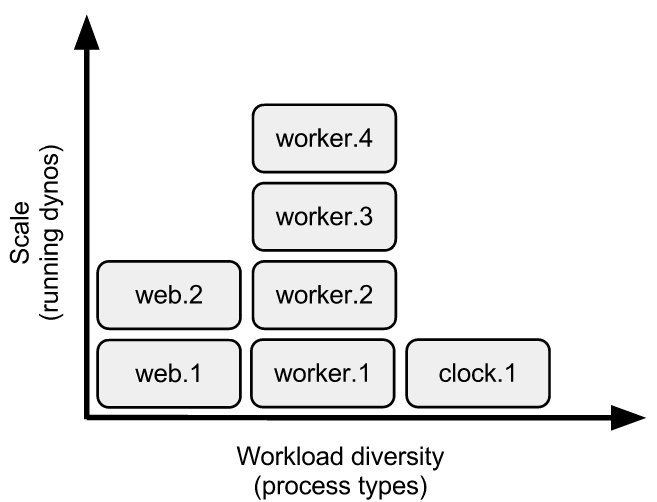
\includegraphics[scale=0.3]{process-type-dyno-relationship.jpg}  
	\caption[Diagram hubungan antara \textit{process type} dan \textit{dyno}]{Diagram hubungan antara \textit{process type} dan \textit{dyno}} 
	\label{fig:process-type-dyno-relationship} 
\end{figure}

\textit{Process type} dan \textit{dyno} saling berhubungan. Hubungan tersebut dapat dilihat pada Gambar~\ref{fig:process-type-dyno-relationship}. Sumbu x menyatakan \textit{process type} yang dipakai, sementara sumbu y menyatakan jumlah \textit{dyno} yang berjalan pada \textit{process type} tersebut. Semakin banyak \textit{dyno} pada suatu \textit{process type} maka konkurensi untuk pekerjaan yang ditangani \textit{process type} tersebut akan meningkat. Semakin banyak \textit{process type} maka semakin beragam beban kerja.

Jumlah \textit{dyno} yang berjalan pada \textit{process type} dapat diatur dengan mengetikkan perintah berikut pada \textit{command shell}:
\begin{lstlisting}
$ heroku ps:scale <process=dyno list>
\end{lstlisting}
Keterangan:
\begin{itemize}
\item \texttt{<process=dyno list>}: daftar pasangan \textit{process type} dengan jumlah \textit{dyno} yang ditugaskan untuk proses tersebut.
\end{itemize}

Contoh: 
\begin{lstlisting}
$ heroku ps:scale web=2 worker=4 clock=1
\end{lstlisting}

\subsubsection{\textit{Dyno}}
\textit{Dyno} adalah wadah aplikasi berbasis Unix yang  menjalankan kode program di Heroku. Pada umumnya, Heroku akan menjalankan satu \textit{web dyno} secara otomatis saat aplikasi disebar ke Heroku untuk pertama kali.

\textit{Dyno} dikelompokkan ke dalam tiga kelompok, yaitu:
\begin{itemize}
\item \textit{Web dyno}

\textit{Web dyno} adalah \textit{dyno} yang berjalan pada \textit{process type} \texttt{web}. \textit{Web dyno} adalah satu-satunya \textit{dyno} yang dapat menerima arus HTTP dari \textit{router} Heroku.

\item \textit{Worker dyno}

\textit{Worker dyno} merujuk kepada \textit{dyno} yang berjalan pada \textit{process type} yang disebutkan di dalam Procfile selain \textit{process type} \texttt{web}. \textit{Worker dyno} biasanya digunakan untuk pekerjaan pada latar belakang, sistem antrian, dan pekerjaan berjangka waktu tertentu.

\item \textit{One-off dyno}

\textit{One-off dyno} adalah \textit{dyno} yang bersifat sementara. \textit{One-off dyno} tidak dituliskan pada Procfile untuk menjalankannya, melainkan menggunakan \textit{command shell}. Contoh penggunaan \textit{one-off dyno} adalah pada saat migrasi basis data.

\end{itemize} 

Heroku menyediakan berbagai macam tipe \textit{dyno}, yaitu: tipe \textit{free}, tipe \textit{hobby}, tipe \textit{standard}, dan tipe \textit{performance}. Tipe \textit{dyno} mempengaruhi karakteristik \textit{dyno} dan kinerja aplikasi. Pada aplikasi dengan tipe \textit{dyno free} dan tipe \textit{dyno hobby}, semua \textit{process type} pada aplikasi tersebut hanya dapat memakai tipe \textit{dyno} tersebut. Namun, tipe \textit{standard} dan tipe \textit{dyno performance} dapat digunakan di aplikasi yang sama. Pada \textit{dyno} tipe \textit{free} dan tipe \textit{hobby}, jumlah \textit{dyno} yang dapat dipakai untuk tiap \textit{process type} adalah satu. Pada tipe \textit{dyno performance}, jumlah \textit{dyno} yang dapat dipakai untuk tiap \textit{process type} adalah sepuluh. Pada tipe \textit{dyno free}, jumlah \textit{dyno} yang dapat dijalankan secara bersamaan pada satu aplikasi adalah dua. Pada tipe \textit{dyno} lainnya, jumlah \textit{dyno} yang dapat dijalankan secara bersamaan pada satu aplikasi adalah seratus.

Tipe \textit{dyno free} memiliki beberapa batasan, yaitu dapat masuk ke kondisi \textit{sleep} dan penggunaan per bulannya dibatasi dengan \textit{free dyno hours}. Kondisi \textit{sleep} adalah kondisi saat \textit{web dyno} tidak aktif. Kondisi \textit{sleep} terjadi apabila tidak ada arus HTTP masuk setelah 30 menit aktif. Apabila ada arus HTTP masuk pada saat aplikasi tertidur, maka aplikasi akan aktif kembali. Namun, ada keterlambatan saat memproses arus HTTP tersebut. \textit{Free dyno hours} adalah jumlah jam saat \textit{web dyno} tidak dalam kondisi \textit{sleep}, saat \textit{worker dyno} berjalan, dan saat \textit{one-off dyno} berjalan. Akun yang belum diverifikasi dapat menggunakan 550 \textit{free dyno hours} tiap bulannya, sedangkan akun yang telah diverifikasi dapat menggunakan 1000 \textit{free dyno hours} tiap bulannya. Setiap aplikasi dengan tipe \textit{dyno free} yang dimiliki pengguna memakai kuota yang sama. Apabila penggunaan \textit{dyno} telah melebihi 80\% kuota, maka pengguna akan dikirimi \textit{email} peringatan. Apabila penggunaan telah melebihi 100\% kuota, maka pengguna akan dikirimi \textit{email} notifikasi kedua dan aplikasinya akan masuk ke kondisi \textit{sleep} selama sisa hari pada bulan tersebut. Jumlah \textit{free dyno hours} yang tersisa dapat dilihat dengan mengetikkan "\texttt{heroku ps -a }" diikuti dengan nama aplikasi di \textit{command shell} atau dengan melihat bagian \textit{free dyno usage} pada halaman billing (\url{https://dashboard.heroku.com/account/billing}).

Perbandingan antar tipe \textit{dyno} dapat dilihat pada Tabel~\ref{table:compare-dyno-type-1} san Tabel~\ref{table:compare-dyno-type-2}. 

\begin{center}
	\begin{table}[H]
	\caption{Tabel perbandingan antar tipe \textit{dyno}}
	\label{table:compare-dyno-type-1}
	\begin{tabular}{|c|c|c|c|}
	\hline
	Tipe \textit{dyno} & \textit{Kondisi sleep} & \textit{Memory} (RAM) & Harga \textit{dyno} per bulan\\
	\hline
	\textit{free} & Ada & 512 MB & \textdollar0\\
	\hline
	\textit{hobby} & Tidak & 512 MB & \textdollar7\\
	\hline
	\textit{standard-1x} & Tidak & 512 MB & \textdollar25\\
	\hline
	\textit{standard-2x} & Tidak & 1024 MB & \textdollar50\\
	\hline
	\textit{performance-m} & Tidak & 2.5 GB & \textdollar250\\
	\hline
	\textit{performance-l} & Tidak & 14 GB & \textdollar500\\
	\hline
	\end{tabular}
	\end{table}
\end{center}

\begin{center}
\begin{table}[H]
\caption{Tabel perbandingan fitur antar tipe \textit{dyno}}
\label{table:compare-dyno-type-2}
\begin{tabular}{|c|p{11cm}|}
\hline
Tipe \textit{dyno} & Fitur\\
\hline
\textit{free} & \begin{itemize}
	\item Mendukung penyebaran aplikasi menggunakan Git dan Docker.
	\item Mengganti \textit{domain}.
	\item Dapat menggunakan \textit{pipeline}\footnotemark
	\item Pembaruan sistem operasi secara berkala.
	\item Pembaruan versi bahasa pemrograman secara berkala.
\end{itemize} \\
\hline
\textit{hobby} & \begin{itemize}
	\item Semua fitur diatas.
	\item Dapat menggunakan SSL dan sertifikat TLS.
	\item Dapat menggunakan \textit{Application metrics}
\end{itemize}\\
\hline
\textit{standard-1x} & \begin{itemize}
	\item Semua fitur diatas.
	\item Dapat menambah jumlah \textit{dyno}.
	\item Dapat mengubah ukuran \textit{dyno}.
	\item Dapat menggunakan fitur \textit{preboot}.
	\item Dapat menggunakan fitur \textit{language runtime metrics}.
\end{itemize}\\
\hline
\textit{standard-2x} & \begin{itemize}
	\item Semua fitur diatas.
\end{itemize}\\
\hline
\textit{performance-m} & \begin{itemize}
	\item Semua fitur diatas.
	\item Dapat menggunakan fitur \textit{autoscaling} untuk \textit{web dynos}
	\item Sumber daya komputasi terdedikasi.
\end{itemize}\\
\hline
\textit{performance-l} & \begin{itemize}
	\item Semua fitur diatas.
\end{itemize}\\
\hline
\end{tabular}
\end{table}
\end{center}
\footnotetext{\textit{Pipeline} adalah sekelompok aplikasi Heroku yang menggunakan kode program yang sama.}

\subsubsection{\textit{Config vars}}
Pada Heroku, \textit{environment variable} disimpan di dalam \textit{config vars}. \textit{Environment variable} adalah konfigurasi yang dapat berubah-ubah pada lingkungan yang berbeda. Konfigurasi tersebut meliputi informasi \textit{database}, informasi kredensial, atau informasi lain yang bersifat spesifik pada aplikasi. Penggunaan \textit{environment variable} dapat menghindari tersimpannya informasi penting di pengontrol versi.

\textit{Config vars} dapat diatur dengan tiga cara : 
\begin{itemize}
\item Menggunakan Heroku CLI

Heroku CLI menggunakan \textit{command shell} untuk menerima perintah yang harus dijalankan. Berikut daftar perintah yang berkaitan dengan \textit{config vars} beserta fungsinya:
\begin{itemize}
\item Menampilkan seluruh \textit{config vars} beserta nilainya : 
\begin{lstlisting}
$ heroku config
\end{lstlisting}

\item Menampilkan nilai dari \textit{config vars} tertentu 
\begin{lstlisting}
$ heroku config : get <config vars>
\end{lstlisting}
Keterangan :
\begin{itemize}
\item \texttt{<config vars>}: nama \textit{config vars}
\end{itemize}

\item Menambah \textit{config vars}
\begin{lstlisting}
$ heroku config : set <config vars> = <config values>
\end{lstlisting}
Keterangan :
\begin{itemize}
\item \texttt{<config vars>}: nama \textit{config vars}
\item \texttt{<config values>}: nilai dari \textit{config vars} tersebut
\end{itemize}

\item Menghapus \textit{config vars}
\begin{lstlisting}
$ heroku config : unset <config vars>
\end{lstlisting}
Keterangan :
\begin{itemize}
\item \texttt{<config vars>} : nama \textit{config vars}
\end{itemize}
\end{itemize}

\item Menggunakan Heroku \textit{Dashboard}
\begin{figure}[H]
	\centering  
	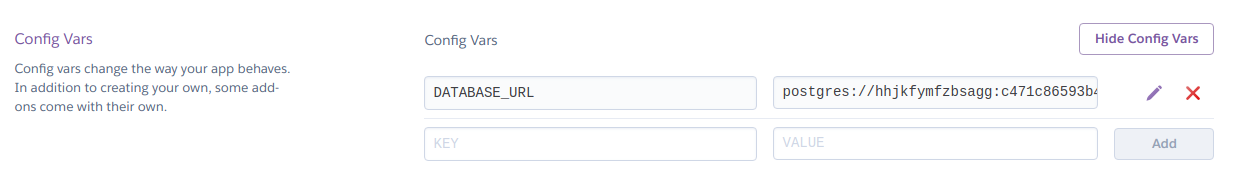
\includegraphics[width=\textwidth]{bluetape-config-vars-example.png}  
	\caption[Config vars pada dashboard Heroku]{Config vars pada dashboard Heroku} 
	\label{fig:bluetape-config-vars-example} 
\end{figure}

Heroku \textit{dashboard} berada di \url{https://dashboard.heroku.com/}. Setelah memilih menu "\texttt{Settings}" di aplikasi yang dipilih, pilih menu "\texttt{Config vars}" untuk melihat, menambah, dan menghapus \textit{config vars}. Tampilan menu "\texttt{Config vars}" dapat dilihat pada Gambar~\ref{fig:bluetape-config-vars-example}.

\item Menggunakan Heroku Platform API

\textit{Config vars} dapat diatur dengan mengirimkan PATCH \textit{request} ke Heroku Platform API dengan format berikut: 
\begin{lstlisting}
PATCH /apps/{app_id_or_name}/config-vars
\end{lstlisting}
Contoh \textit{request} menggunakan curl:
\begin{lstlisting}
$ curl -n -X PATCH https://api.heroku.com/apps/$APP_ID_OR_NAME/config-vars \
	-d '{
	"FOO": "bar",
	"BAZ": "qux"
}' \
	-H "Content-Type: application/json" \
	-H "Accept: application/vnd.heroku+json; version=3"
\end{lstlisting}
Contoh \textit{response} dari Heroku Platform API:
\begin{lstlisting}
HTTP/1.1 200 OK
ETag: "0123456789abcdef0123456789abcdef"
Last-Modified: Sun, 01 Jan 2012 12:00:00 GMT
RateLimit-Remaining: 4500
{
  "FOO": "bar",
  "BAZ": "qux"
}
\end{lstlisting}

Apabila pengguna ingin melihat \textit{config vars}, maka pengguna dapat mengirimkan GET \textit{request} dengan format berikut: 
\begin{lstlisting}
GET /apps/{app_id_or_name}/config-vars
\end{lstlisting}
Contoh \textit{request} menggunakan curl:
\begin{lstlisting}
$ curl -n https://api.heroku.com/apps/$APP_ID_OR_NAME/config-vars \
-H "Accept: application/vnd.heroku+json; version=3"
\end{lstlisting}
Contoh \textit{response} dari Heroku Platform API:
\begin{lstlisting}
HTTP/1.1 200 OK
ETag: "0123456789abcdef0123456789abcdef"
Last-Modified: Sun, 01 Jan 2012 12:00:00 GMT
RateLimit-Remaining: 4500
{
  "FOO": "bar",
  "BAZ": "qux"
}
\end{lstlisting}
\end{itemize}

Dalam mengatur \textit{config vars}, ada beberapa hal yang harus diperhatikan:
\begin{itemize}
\item Setiap \textit{config vars} ditambah atau dihapus, aplikasi akan dimulai ulang dan \textit{release} baru akan dibuat.
\item Jika aplikasi menggunakan \textit{add-ons}, biasanya \textit{add-ons} tersebut akan menambahkan satu atau lebih \textit{config vars} ke aplikasi. Nilai dari \textit{config vars} tersebut mungkin diperbarui oleh penyedia \textit{add-ons} kapan saja.
\item Data \textit{config vars} (kombinasi dari semua kunci dan nilainya) tidak dapat melebihi 32 kb per aplikasi
\item Nama \textit{config vars} tidak boleh diawali dengan tanda hubung bawah dua kali (\texttt{\_\_}).
\item Nama \textit{config vars} tidak bisa diawali dengan \texttt{HEROKU\_}, kecuali ditambahkan oleh platform Heroku sendiri.
\end{itemize}

\subsubsection{\textit{Add-ons}}
Pengguna Heroku dapat memanfaatkan \textit{add-ons} untuk memakai layanan penyokong, misalnya basis data, sistem antrean, layanan \textit{email}, dan lain-lain. Pengguna Heroku dapat mencari \textit{add-ons} di situs web \textit{Elements Marketplace} (\url{https://elements.heroku.com/addons}). Beberapa \textit{add-ons} di dalam situs web tersebut disediakan oleh Heroku dan beberapa lainnya disediakan oleh pihak ketiga. Pengguna Heroku dapat memasang \textit{add-ons} pada aplikasi dengan menekan tombol "\texttt{Install}" di situs web \textit{Elements Marketplace} atau dengan mengetikkan perintah berikut pada \textit{command shell} :
\begin{lstlisting}
$ heroku addons:create <nama add-ons>:<tipe add-ons>
\end{lstlisting}
Keterangan:
\begin{itemize}
\item \texttt{<nama add-ons>} : nama \textit{add-ons}
\item \texttt{<tipe add-ons>} : tipe \textit{add-ons}
\end{itemize}
Contoh:
\begin{lstlisting}
$ heroku addons:create heroku-redis:hobby-dev
\end{lstlisting}

Menambah \textit{add-ons} selain \textit{add-ons} Heroku Postgres dan Heroku Connect membutuhkan verifikasi akun.

\subsubsection{\textit{Slug}}
\textit{Slug} adalah gabungan dari \textit{source code}, \textit{dependency}, \textit{language runtime}, dan hasil \textit{build} yang siap untuk dijalankan. \textit{Slug} dibuat oleh \textit{buildpack} setiap pengguna melakukan \textit{deploy}. Ukuran maksimal \textit{slug} adalah 500 MB. Waktu pembuatan \textit{slug} dibatasi sampai 15 menit. Agar waktu pembuatan \textit{slug} lebih singkat, pengguna dapat mengecualikan \textit{file} yang tidak diperlukan untuk menjalankan aplikasi dengan menuliskannya di dalam \textit{file} \texttt{.slugignore}. \textit{File} \texttt{.slugignore} adalah \textit{file} yang menyebutkan \textit{file} yang harus diabaikan pada saat pembuatan \textit{slug}. \textit{File} ini diletakkan di direktori \texttt{root}. Cara penulisan \texttt{.slugignore} kurang lebih sama dengan \textit{.gitignore}. Contoh isi \texttt{.slugignore}:
\begin{lstlisting}
# Heres a comment
*.psd
*.pdf
/test
/spec
\end{lstlisting}

\subsubsection{\textit{Buildpack}}
\begin{figure}[H]
	\centering  
	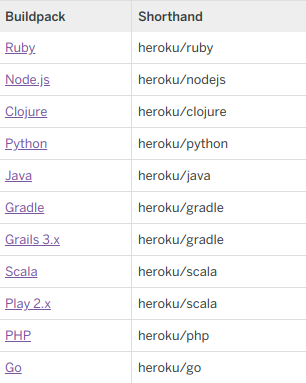
\includegraphics[scale=0.5]{heroku-buildpack-table.png}  
	\caption[Tabel buildpack heroku]{Tabel buildpack heroku} 
	\label{fig:heroku-buildpack-table} 
\end{figure}

\textit{Buildpack} adalah kumpulan kode program yang bertugas untuk mengubah \textit{source code} menjadi \textit{slug}, sehingga \textit{dyno} dapat mengeksekusinya. Heroku biasanya akan secara otomatis menugaskan \textit{buildpack} yang akan dipakai setelah \textit{build} pertama berhasil. Daftar \textit{buildpack} yang tersedia di Heroku dapat dilihat pada Gambar~\ref{fig:heroku-buildpack-table}. Kolom \texttt{Buildpack} menyatakan nama \textit{buildpack} dan kolom \texttt{shorthand} menyatakan nama panggil \textit{buildpack} di Heroku CLI.

Jumlah \textit{buildpack} yang dipakai oleh satu aplikasi biasanya hanya satu, tapi ada beberapa kasus \textit{buildpack} yang dipakai lebih dari satu. Contoh kasus \textit{buildpack} tambahan dibutuhkan:
\begin{itemize}
\item Satu aplikasi memiliki lebih dari satu bahasa pemrograman.
\item Aplikasi menjalankan \textit{daemon}.
\item Aplikasi membutuhkan \textit{dependency} yang diambil dengan \textit{APT (Advanced Package Tool)}.
\end{itemize}

\textit{Buildpack} dapat diatur dengan mengetikkan perintah di \textit{command shell} menggunakan Heroku CLI. Berikut daftar perintah yang berkaitan dengan \textit{buildpack} beserta fungsinya:
\begin{itemize}
\item Mengatur \textit{buildpack} yang dipakai saat aplikasi pertama kali dibuat:
\begin{lstlisting}
$ heroku create myapp --buildpack <nama buildpack>
\end{lstlisting}
Keterangan:
\begin{itemize}
\item \texttt{<nama buildpack>}: nama panggil \textit{buildpack}, contoh: \texttt{heroku/php}.
\end{itemize}
\item Mengubah dengan mengatur nilai \textit{buildpack}:
\begin{lstlisting}
$ heroku buildpacks:set <nama buildpack>
\end{lstlisting}
Keterangan:
\begin{itemize}
\item \texttt{<nama buildpack>}: nama panggil \textit{buildpack}, contoh: \texttt{heroku/php}.
\end{itemize}
\item Menghilangkan \textit{buildpack} dari aplikasi:
\begin{lstlisting}
$ heroku buildpacks:remove <nama buildpack>
\end{lstlisting}
Keterangan:
\begin{itemize}
\item \texttt{<nama buildpack>}: nama panggil \textit{buildpack}, contoh: \texttt{heroku/php}.
\end{itemize}
\item Mencari buildpack:
\begin{lstlisting}
$ heroku buildpacks:search <kata kunci>
\end{lstlisting}
Keterangan:
\begin{itemize}
\item \texttt{<kata kunci>}: kata kunci pencarian, misalnya nama bahasa pemrograman. Contoh kata kunci: \texttt{elixir}.
\end{itemize}
\item Menampilkan informasi \textit{buildpack}:
\begin{lstlisting}
$ heroku buildpacks:info <nama buildpack>	
\end{lstlisting}
Keterangan:
\begin{itemize}
\item \texttt{<nama buildpack>}: nama panggil \textit{buildpack}, contoh: \texttt{heroku/php}.
\end{itemize}
\item Mengembalikan aplikasi ke \textit{buildpack} awalnya:
\begin{lstlisting}
$ heroku buildpacks:clear	
\end{lstlisting}
\item Mengatur urutan eksekusi \textit{buildpack}:
\begin{lstlisting}
$ heroku buildpacks:set --index <index> <nama buildpack>
\end{lstlisting}
Keterangan:
\begin{itemize}
\item \texttt{<index>}: urutan eksekusi \textit{buildpack}
\item \texttt{<nama buildpack>}: nama panggil \textit{buildpack}, contoh : \texttt{heroku/php}.
\end{itemize}
\item Melihat daftar \textit{buildpack} yang dipakai pada satu aplikasi:
\begin{lstlisting}
$ heroku buildpacks
\end{lstlisting}
\end{itemize}

\subsubsection{\textit{Stack}}
\textit{Stack} merujuk pada sistem operasi yang dikelola dan dipelihara oleh Heroku. \textit{Stack} biasanya memakai sistem operasi Linux, misalnya Ubuntu. Saat skripsi ini dibuat, Heroku menyediakan tiga pilihan \textit{stack}: \texttt{Cedar-14}, \texttt{Heroku-16}, dan \texttt{Heroku-18}. Perbandingan ketiga \textit{stack} tersebut dapat dilihat di Tabel~\ref{table:compare-stack}.
\begin{center}
	\begin{table}[H]
	\caption{Tabel perbandingan antar \textit{stack}}
	\label{table:compare-stack}
	\begin{tabular}{|c|c|c|}
	\hline
	Nama \textit{stack} & Sistem Operasi yang dipakai & Periode dukungan\\
	\hline
	\texttt{Cedar-14} & Ubuntu 14.04 & Sampai bulan April 2019\\
	\hline
	\texttt{Heroku-16} & Ubuntu 16.04 & Sampai bulan April 2021\\
	\hline
	\texttt{Heroku-18} & Ubuntu 18.04 & Sampai bulan April 2023\\
	\hline
	\end{tabular}
	\end{table}
\end{center}
Pengguna Heroku dapat melihat \textit{stack} yang dipakai pada suatu aplikasi dengan mengetikkan perintah berikut pada \textit{command shell}:
\begin{lstlisting}
$ heroku stack
\end{lstlisting}
Pada saat aplikasi baru dibentuk, Heroku akan secara otomatis memakai \textit{stack} yang memiliki periode dukungan paling panjang. Namun, pengguna dapat mengganti \textit{stack} yang dipakai dengan mengetikkan perintah berikut pada \textit{command shell}:
\begin{lstlisting}
$ heroku stack:set <stack>
\end{lstlisting}
Keterangan:
\begin{itemize}
\item \texttt{<stack>}: nama \textit{stack}, contoh: \texttt{cedar-14}.
\end{itemize}

\subsubsection{\textit{Region}}
Aplikasi yang ada di Heroku dapat disebarkan ke lokasi geografis yang berbeda. Pada heroku, lokasi penyebaran aplikasi disebut \textit{region}. \textit{Region} yang tersedia untuk pengguna Heroku yang merupakan perorangan adalah lokasi dengan \textit{runtime Common Runtime}, sedangkan \textit{region} yang tersedia untuk pengguna Heroku yang merupakan badan bisnis (Heroku Enterprise) adalah lokasi dengan \textit{runtime Private Space}. Pada saat skripsi ini dibuat, pengguna Heroku yang merupakan perorangan hanya dapat memilih antara \textit{Europe} (Eropa) dan \textit{United States} (Amerika Serikat). Apabila pengguna tidak memilih \textit{region} saat membuat aplikasi, maka Heroku akan secara otomatis mengatur \textit{region} menjadi \textit{United States}. Beberapa layanan yang disediakan untuk membangun aplikasi di Heroku hanya dapat digunakan di \textit{region} tertentu, sehingga pengguna lebih baik merencanakannya terlebih dahulu sebelum memilih \textit{region}.

Berikut perintah-perintah penting yang berkaitan dengan \textit{region} yang dapat diketikkan pada \textit{command shell} :
\begin{itemize}
\item Memeriksa \textit{region} yang tersedia di Heroku:
\begin{lstlisting}
$ heroku regions
\end{lstlisting}
\item Mengatur \textit{region} aplikasi:
\begin{lstlisting}
$ heroku create --region <id region>
\end{lstlisting}
Keterangan:
\begin{itemize}
\item \texttt{<id region>}: \textit{id region} yang ingin dipakai, contoh: \texttt{eu}. \textit{Id region} bisa dilihat dengan memeriksa daftar region yang tersedia.
\end{itemize}
\item Memeriksa \textit{region} yang dipakai oleh aplikasi:
\begin{lstlisting}
$ heroku info
\end{lstlisting}
\end{itemize}

\subsubsection{\textit{Releases}}
Setiap pengguna melakukan \textit{deploy}, merubah \textit{config vars}, dan merubah daftar \textit{add-ons} yang dipakai, Heroku akan mencatat aktivitas tersebut di \textit{releases}. \textit{Releases} adalah buku besar yang mencatat setiap ada perubahan baru pada aplikasi. \textit{Releases} berbentuk tabel yang memiliki empat kolom, yaitu \textit{"Rel", "Change", "By",} dan \textit{"When"}. Kolom"\textit{rel}" berisi versi aplikasi, kolom "\textit{Change}" berisi keterangan singkat perubahan yang terjadi, kolom "\textit{By}" berisi alamat \textit{email} pengguna yang melakukan perubahan, dan kolom "When" berisi waktu perubahan tersebut terjadi. Pengguna dapat melihat \textit{releases} dengan mengetikkan perintah berikut di \textit{command shell}:
\begin{lstlisting}
$ heroku releases
\end{lstlisting}

Berikut contoh isi \textit{releases}:
\begin{lstlisting}
Rel   Change                          By                    When
----  ----------------------          ----------            ----------
v52   Config add AWS_S3_KEY           jim@example.com       5 minutes ago
v51   Deploy de63889                  stephan@example.com   7 minutes ago
v50   Deploy 7c35f77                  stephan@example.com   3 hours ago
v49   Rollback to v46                 joe@example.com       2010-09-12 15:32:17 -0700
\end{lstlisting}

Releases berguna ketika pengguna ingin mengembalikan aplikasi ke versi tertentu. Cara mengembalikan aplikasi ke versi tertentu adalah dengan mengetikkan perintah berikut pada \textit{command shell}:
\begin{lstlisting}
$ heroku releases:rollback <version>
\end{lstlisting}
Keterangan:
\begin{itemize}
\item \texttt{<version>}: Versi aplikasi
\end{itemize}

\subsubsection{\textit{Log}}
\textit{Log} adalah catatan setiap proses yang terjadi di aplikasi. Heroku menggunakan Logplex untuk menyampaikan \textit{log} ini. Logplex akan secara otomatis menambahkan entri \textit{log} baru dari semua \textit{dyno} yang berjalan di aplikasi, dan juga komponen lain seperti \textit{router}. Pengguna dapat melihat \textit{log} dengan cara mengetikkan perintah berikut pada \textit{command shell}:
\begin{lstlisting}
$ heroku logs
\end{lstlisting}

Isi \textit{log} memiliki format sebagai berikut:
\begin{lstlisting}
<timestamp> <source>[<dyno>]: <message>
\end{lstlisting}
Keterangan:
\begin{itemize}
\item \texttt{<timestamp>}: Waktu \textit{log} dicatat dengan tingkat ketelitian hingga mikrodetik.
\item \texttt{<source>}: Jika \textit{log} berasal dari \textit{dyno}, maka isinya adalah "\texttt{app}". Jika \textit{log} berasal dari komponen sistem Heroku (HTTP \textit{router, dyno manager}) maka isinya adalah "\texttt{heroku}".
\item \texttt{dyno}: Nama \textit{dyno} atau komponen yang dicatat di \textit{log}.
\item \texttt{message}: Keterangan \textit{log}.
\end{itemize}

Berikut contoh isi \textit{log}:
\begin{lstlisting}
2010-09-16T15:13:46.677020+00:00 app[web.1]: Processing PostController#list (for 208.39.138.12 at 2010-09-16 15:13:46) [GET]
2010-09-16T15:13:46.677023+00:00 app[web.1]: Rendering template within layouts/application
2010-09-16T15:13:46.677902+00:00 app[web.1]: Rendering post/list
2010-09-16T15:13:46.678990+00:00 app[web.1]: Rendered includes/_header (0.1ms)
2010-09-16T15:13:46.698234+00:00 app[web.1]: Completed in 74ms (View: 31, DB: 40) | 200 OK [http://myapp.heroku.com/]
2010-09-16T15:13:46.723498+00:00 heroku[router]: at=info method=GET path="/posts" host=myapp.herokuapp.com" fwd="204.204.204.204" dyno=web.1 connect=1ms service=18ms status=200 bytes=975
2010-09-16T15:13:47.893472+00:00 app[worker.1]: 2 jobs processed at 16.6761 j/s, 0 failed ...
\end{lstlisting}

Heroku mengelompokkan \textit{log} ke dalam empat kelompok:
\begin{itemize}
\item \textit{App logs}

\textit{Log} yang berasal dari aplikasi, termasuk \textit{log} yang dihasilkan oleh kode program dan \textit{dependency}. Pengguna dapat melihat \textit{app logs} dengan cara mengetikkan perintah berikut pada \textit{command shell}:
\begin{lstlisting}
$ heroku logs --source app
\end{lstlisting}

\item \textit{System Logs}

\textit{Log} yang berisi pesan tentang tindakan yang diambil oleh infrastruktur Heroku mewakili aplikasi, misalnya: saat terjadi \textit{error}. Pengguna dapat melihat \textit{system logs} dengan cara mengetikkan perintah berikut pada \textit{command shell}:
\begin{lstlisting}
$ heroku logs --source heroku
\end{lstlisting}

\item \textit{API logs} 

\textit{Log} yang berisi pesan tentang tindakan administratif yang diambil oleh pembuat aplikasi, misalnya: saat melakukan \textit{deploy}. Pengguna dapat melihat \textit{API logs} dengan cara mengetikkan perintah berikut pada \textit{command shell}:
\begin{lstlisting}
$ heroku logs --source app --dyno api
\end{lstlisting}

\item \textit{Add-on logs}

\textit{Log} yang berisi pesan dari layanan \textit{add-ons}.
\end{itemize}

Pengguna Heroku dapat menuliskan \textit{log} dengan cara megirimkan pesan ke \textit{standard out (stdout)} atau \textit{standard error (stderr)}. Cata mengirimkannya berbeda-beda tergantung bahasa pemrograman yang dipakai. Pada bahasa PHP, \textit{log} dapat dikirim dengan menggunakan fungsi "\texttt{error\_log}" atau menulis ke "\texttt{php://stderr}".

Contoh penggunaan fungsi "\texttt{error\_log}":
\begin{lstlisting}
error_log("hello, this is a test!");
\end{lstlisting}

Contoh menulis ke "\texttt{php://stderr}":
\begin{lstlisting}
file_put_contents("php://stderr", "hello, this is a test!\n");
\end{lstlisting}

Apabila aplikasi menggunakan \textit{framework} Codeigniter, maka pembuat aplikasi perlu menambahkan \textit{file} \texttt{application/core/MY\_Log.php} dan mengatur "\texttt{sub-class prefix}" menjadi "\texttt{MY\_}". Isi \textit{file} tersebut adalah sebagai berikut:

\begin{lstlisting}
<?php  if ( ! defined('BASEPATH')) exit('No direct script access allowed');

// this class is adapted from system/libraries/Log.php
/**
 * CodeIgniter
 *
 * An open source application development framework for PHP 5.1.6 or newer
 *
 * @package     CodeIgniter
 * @author      EllisLab Dev Team
 * @copyright       Copyright (c) 2008 - 2014, EllisLab, Inc.
 * @copyright       Copyright (c) 2014 - 2015, British Columbia Institute of Technology (http://bcit.ca/)
 * @license     http://codeigniter.com/user_guide/license.html
 * @link        http://codeigniter.com
 * @since       Version 1.0
 * @filesource
 */

// ------------------------------------------------------------------------

/**
 * Logging Class
 *
 * @package     CodeIgniter
 * @subpackage  Libraries
 * @category    Logging
 * @author      EllisLab Dev Team
 * @link        http://codeigniter.com/user_guide/general/errors.html
 */
class MY_Log {

    protected $_threshold   = 1;
    protected $_date_fmt    = 'Y-m-d H:i:s';
    protected $_levels  = array('ERROR' => '1', 'DEBUG' => '2',  'INFO' => '3', 'ALL' => '4');

    /**
     * Constructor
     */
    public function __construct()
    {
        $config =& get_config();

        if (is_numeric($config['log_threshold']))
        {
            $this->_threshold = $config['log_threshold'];
        }

        if ($config['log_date_format'] != '')
        {
            $this->_date_fmt = $config['log_date_format'];
        }
    }

    // --------------------------------------------------------------------

    /**
     * Write Log to php://stderr
     *
     * Generally this function will be called using the global log_message() function
     *
     * @param   string  the error level
     * @param   string  the error message
     * @param   bool    whether the error is a native PHP error
     * @return  bool
     */
    public function write_log($level = 'error', $msg, $php_error = FALSE)
    {
        $level = strtoupper($level);

        if ( ! isset($this->_levels[$level]) OR ($this->_levels[$level] > $this->_threshold))
        {
            return FALSE;
        }

        file_put_contents('php://stderr', $level.' '.(($level == 'INFO') ? ' -' : '-').' '.date($this->_date_fmt). ' --> '.$msg."\n");

        return TRUE;
    }

}
// END Log Class

/* End of file MY_Log.php */
/* Location: ./application/core/MY_Log.php */
\end{lstlisting}

\subsection{\textit{Deploy} Perangkat Lunak}
Heroku menggunakan Git sebagai sarana  utama untuk melakukan \textit{deploy} ke Heroku. Deploy adalah proses penyebaran aplikasi dari satu lingkungan ke lingkungan lain, misalnya dari lingkungan lokal aplikasi ke lingkungan Heroku. Namun, Heroku juga menyediakan cara lain untuk melakukan \textit{deploy}:
\begin{itemize}
\item Docker
\item GitHub
\item Tombol \texttt{Deploy} di dashboard Heroku
\item WAR deployment
\end{itemize}

\subsubsection{\textit{Deploy} Menggunakan Git}
\textit{Deploy} dengan Git dapat dilakukan apabila Git telah terpasang. Git dapat dipasang dengan mengikuti petunjuk unduhan pada \url{https://git-scm.com}. Sebelum \textit{deploy} dengan Git dapat dilakukan, Git perlu diinisialisasi terlebih dahulu dengan mengetikkan perintah berikut pada \textit{command shell} :
\begin{lstlisting}
$ git init
\end{lstlisting}

Setelah melakukan inisialisasi Git, aplikasi Heroku dapat dibuat. Setiap aplikasi Heroku dibuat, maka \texttt{git remote} secara otomatis juga dibuat. Nama \textit{remote} dapat diperiksa dengan mengetikkan perintah berikut pada \textit{command shell} :
\begin{lstlisting}
$ git remote
\end{lstlisting}

Nama \textit{remote} dapat diubah dengan mengetikkan perintah berikut pada \textit{command shell} :
\begin{lstlisting}
$ git remote rename <nama lama> <nama baru>
\end{lstlisting}
Keterangan:
\begin{itemize}
\item \texttt{<nama lama>}: nama \textit{remote} yang ingin diganti.
\item \texttt{<nama baru>}: nama baru untuk \textit{remote} tersebut.
\end{itemize}

Deploy dapat dimulai dengan mengetikkan perintah berikut pada \textit{command shell} :
\begin{lstlisting}
$ git add <nama file>
$ git commit -m "<message>"
$ git push <nama remote> <nama branch>
\end{lstlisting}
Keterangan :
\begin{itemize}
\item \texttt{<nama file>}: nama \textit{file} yang telah diubah. Menulis tanda titik untuk nama \textit{file} mewakili semua \textit{file} yang telah berubah.
\item \texttt{<message>}: pesan yang menerangkan hal yang ingin disebar.
\item \texttt{<nama remote>} : nama remote dari tujuan deploy. Bila \textit{developer} tidak mengubah nama remote, nama remotenya adalah \texttt{heroku}. 
\item \texttt{<nama branch>} : nama cabang dari tujuan deploy. Heroku secara otomatis membuat satu cabang bernama \texttt{master}.
\end{itemize}

\subsubsection{\textit{Deploy} Menggunakan Docker}
\textit{Deploy} dengan Docker dapat dilakukan apabila Docker telah terpasang dan pengguna Heroku telah masuk ke akun Heroku. Langkah-langkah untuk melakukan \textit{deploy} menggunakan Docker adalah sebagai berikut:
\begin{itemize}
\item Masuk ke \textit{Container Registry} dengan mengetikkan perintah berikut pada \textit{command shell}:
\begin{lstlisting}
$ heroku container:login
\end{lstlisting}

\item \textit{Clone source code} contoh dari Alpine dengan mengetikkan perintah berikut pada \textit{command shell}:
\begin{lstlisting}
$ git clone https://github.com/heroku/alpinehelloworld.git
\end{lstlisting}

\item Membuat aplikasi Heroku baru dengan mengetikkan perintah berikut pada \textit{command shell}:
\begin{lstlisting}
$ heroku create
\end{lstlisting}

\item Membangun \textit{image} dan melakukan \textit{deploy} ke \textit{Container Registry} dengan mengetikkan perintah berikut pada \textit{command shell}:
\begin{lstlisting}
$ heroku container:push web
\end{lstlisting}

\item Melepaskan \textit{image} ke aplikasi dengan mengetikkan perintah berikut pada \textit{command shell}:
\begin{lstlisting}
$ heroku container:release web
\end{lstlisting}

\item Membuka aplikasi dengan mengetikkan perintah berikut pada \textit{command shell}:
\begin{lstlisting}
$ heroku open
\end{lstlisting}
\end{itemize}

\subsubsection{\textit{Deploy} Menggunakan GitHub}
\begin{figure}[H]
	\centering  
	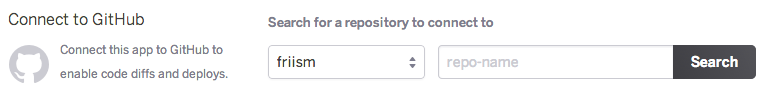
\includegraphics[scale=0.5]{deploy-github-dashboard.jpg}  
	\caption[\textit{Deploy} menggunakan Github \textit{Dashboard}]{\textit{Deploy} menggunakan Github \textit{Dashboard}} 
	\label{fig:deploy-github-dashboard} 
\end{figure}
\textit{Deploy} dengan cara ini membuat Heroku melakukan \textit{deploy} secara otomatis ke GitHub apabila \textit{build} berhasil. \textit{Deploy} ini dapat dilakukan apabila GitHub \textit{integration} telah aktif dan akun Github telah terautentikasi pada Heroku. Autentikasi ini hanya perlu dilakukan satu kali per satu akun Heroku. Setelah kedua hal tersebut telah siap, sambungkan \textit{repository} Github dengan aplikasi Heroku. (Gambar~\ref{fig:deploy-github-dashboard}).

\begin{figure}[H]
	\centering  
	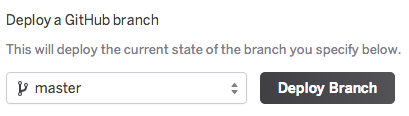
\includegraphics[scale=0.5]{deploy-github-manual.jpg}  
	\caption[\textit{Deploy} menggunakan Github secara manual]{\textit{Deploy} menggunakan Github secara manual} 
	\label{fig:deploy-github-manual} 
\end{figure}
\begin{figure}[H]
	\centering  
	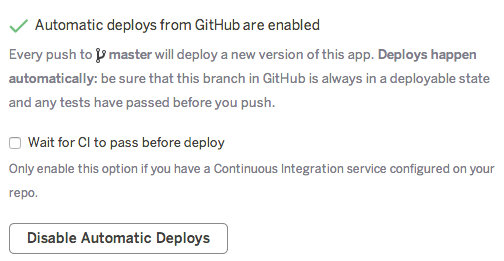
\includegraphics[scale=0.5]{deploy-github-automatic.jpg}  
	\caption[\textit{Deploy} menggunakan Github secara otomatis]{\textit{Deploy} menggunakan Github secara otomatis} 
	\label{fig:deploy-github-automatic} 
\end{figure}
Ada dua cara untuk melakukan deploy, yaitu secara manual dan secara otomatis. Untuk cara manual, \textit{deploy} dilakukan dari GitHub (Gambar~\ref{fig:deploy-github-manual}). Untuk cara otomatis, \textit{deploy} dilakukan dengan mengaktifkan "\textit{Automatic deploys from GitHub}" (Gambar~\ref{fig:deploy-github-automatic}).

\subsubsection{Deploy Langsung di situs web Heroku}
Pada situs web Heroku, tombol "\textit{Deploy to Heroku}" memungkinkan pengguna untuk melakukan deploy aplikasi tanpa meninggalkan situs web Heroku. Cara ini hampir tidak memerlukan konfigurasi. Sebelum dapat melakukan \textit{deploy} dengan cara ini, aplikasi harus memiliki \textit{file} \texttt{app.json} yang sah pada direktori \texttt{root}, dan \textit{source code} aplikasi harus berada di \textit{repository} GitHub.

\texttt{app.json} adalah \textit{file} berisi deskripsi aplikasi \textit{web}. Isinya dapat berupa \textit{environment variable, add-ons}, dan informasi lain yang diperlukan untuk menjalankan aplikasi pada Heroku. Heroku tidak mewajibkan penulisan informasi tertentu, tapi Heroku merekomendasikan untuk setidaknya menuliskan nama aplikasi(\texttt{name}), deskripsi aplikasi (\texttt{description}), dan logo aplikasi (\texttt{logo}). Berikut contoh isi dari \texttt{app.json} :
\begin{lstlisting}
{
  "name": "Node.js Sample",
  "description": "A barebones Node.js app using Express 4",
  "repository": "https://github.com/heroku/node-js-sample",
  "logo": "https://node-js-sample.herokuapp.com/node.png",
  "keywords": ["node", "express", "static"]
}
\end{lstlisting}

\subsubsection{\textit{WAR Deployment}}
\textit{WAR (Web Application Archive)} adalah jenis \textit{file} arsip yang digunakan untuk membungkus aplikasi \textit{web}. Dokumen ini dapat berisi halaman \textit{web} statis, \textit{file} XML, dan lain-lain. \cite{etzkorn2017introduction}

\textit{WAR deployment} dapat dilakukan menggunakan \textit{plugin} Heroku Java CLI Plugin. Pemasangan dan pembaruan \textit{plugin} ini dapat dilakukan dengan mengetikkan perintah berikut pada \textit{command shell}:
\begin{lstlisting}
heroku plugins:install java
\end{lstlisting}

\textit{Deploy} dapat dilakukan dengan mengetikkan perintah berikut pada \textit{command shell}:
\begin{lstlisting}
heroku war:deploy <path_to_war_file> --app <app_name>
\end{lstlisting}
Keterangan:
\begin{itemize}
\item \texttt{<path\_to\_war\_file>}: letak \textit{file} WAR.
\item \texttt{<app\_name>}: nama aplikasi.
\end{itemize}

\subsection{\textit{Ephemereal Filesystem}}
Heroku memiliki \textit{ephemereal filesystem}, yang berarti perubahan apapun pada \textit{file} di lingkungan Heroku tidak akan disimpan secara permanen. Kondisi \textit{file} di Heroku akan selalu dikembalikan ke \textit{deploy baru}. Perubahan \textit{file} hanya akan bertahan paling lama satu hari. Kondisi ini membuat aplikasi di Heroku membutuhkan layanan dari pihak ketiga untuk menyimpan hasil unggahan pengguna aplikasi.

\subsection{Basis Data dan Manajemen Data}
Heroku menyediakan tiga layanan data untuk semua pelanggan :
\begin{itemize}
\item Heroku Postgres
\item Heroku Redis
\item Apache Kafka
\end{itemize}
Heroku juga menyediakan pilihan lain untuk pengguna Heroku Enterprise, yaitu Heroku Connect. Selain itu, Heroku juga memungkinkan penggunaan layanan data dari pihak ketiga. Layanan data dari pihak ketiga ini tersedia sebagai add-ons.

\subsubsection{Heroku Postgres}
Heroku Postgres adalah basis data SQL yang disediakan secara langsung oleh Heroku. Heroku Postgres dapat diakses oleh bahasa apapun dengan PostgreSQL \textit{driver}. Heroku secara otomatis membuat satu basis data menggunakan \textit{add-ons} Heroku Postgres setiap aplikasi dibuat. Perintah berikut dapat diketikkan pada \textit{command shell} apabila ingin menambah basis data baru:
\begin{lstlisting}
$ heroku addons:create heroku-postgresql:<PLAN_NAME>
\end{lstlisting}
Keterangan :
\begin{itemize}
\item \texttt{<PLAN\_NAME>} : nama \textit{plan} Heroku Postgres yang ingin dipakai. Heroku secara otomatis menggunakan Heroku Postgres tipe \texttt{hobby-dev}.
\end{itemize}

Heroku menawarkan lima \textit{plan} untuk Heroku Postgres, yaitu:
\begin{itemize}
\item Hobby Tier: \textit{plan} dengan toleransi gagal bekerja sampai 4 jam per bulan.
\item Standard Tier: \textit{plan} dengan toleransi gagal bekerja sampai 1 jam per bulan.
\item Premium Tier: \textit{plan} dengan toleransi gagal bekerja sampai 15 menit per bulan.
\item Private Tier: \textit{plan} yang dapat dipilih oleh pengguna Heroku \textit{Enterprise}, memiliki toleransi gagal bekerja sampai 15 menit per bulan.
\item Shield Tier : \textit{plan} yang dapat dipilih oleh pengguna Heroku \textit{Enterprise}, memiliki toleransi gagal bekerja sampai 15 menit per bulan. Kelebihannya daripada \textit{Private Tier} adalah basis data ini memiliki keamanan yang lebih ketat.
\end{itemize}

Gambar~\ref{fig:heroku-postgres-plan-table} menunjukkan tabel perbandingan antar \textit{plan}. Di antara lima \textit{plan} Heroku Postgres, hanya \textit{plan Hobby} yang gratis. \textit{Plan} lain memiliki harga yang bervariasi berdasarkan ukuran RAM, batas penyimpanan, dan batas koneksi yang bisa dibuat.
\begin{figure}[H]
	\centering  
	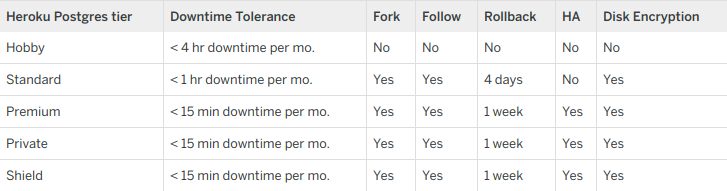
\includegraphics[scale=0.5]{heroku-postgres-plan-table.png}  
	\caption[Tabel plan Heroku Postgres]{Tabel plan Heroku Postgres} 
	\label{fig:heroku-postgres-plan-table} 
\end{figure}

Semua \textit{plan} memiliki fitur yang sama:
\begin{itemize}
\item Dikelola secara otomatis oleh Heroku.
\item Data dijamin tidak akan hilang.
\item Dapat melakukan \textit{backup} basis data secara harian menggunakan Heroku PGBackups.
\item Dapat menggunakan layanan Dataclips (\url{https://data.heroku.com/dataclips}) untuk berbagi data dan \textit{query}.
\item Akses basis data diproteksi dengan SSL.
\item Menjalankan Postgres versi 9.4, 9.5, 9.6, atau 10 tanpa modifikasi
\item Tersedia ekstensi Postgres
\item Memiliki tampilan \textit{web} yang dapat diakses pada situs web \url{https://data.heroku.com/}
\end{itemize}

\textit{Developer} juga dapat menambahkan versi yang ingin dipakai dengan cara menambahkan \texttt{--version} di belakang perintah tersebut, contoh :
\begin{lstlisting}
$ heroku addons:create heroku-postgresql:<PLAN_NAME--version=9.5
\end{lstlisting}
Secara otomatis, Heroku menggunakan versi paling baru dari Heroku Postgres. Saat skripsi ini ditulis, versi terbaru adalah versi 10.

Setelah dipasang, Heroku akan secara otomatis menambahkan \textit{config vars} \texttt{DATABASE\_URL} ke aplikasi. Apabila Heroku Postgres yang dipakai ada lebih dari satu, nama \textit{config vars} akan menjadi \texttt{HEROKU\_POSTGRESQL\_<COLOR>\_URL} dengan <COLOR> adalah nama warna yang dihasilkan secara acak oleh Heroku. Contoh: \texttt{HEROKU\_POSTGRESQL\_<BLUE>\_URL}.

Apabila basis data yang digunakan lebih dari satu, basis data utama dapat diatur dengan mengetikkan perintah berikut pada \textit{command shell}:
\begin{lstlisting}
$ heroku pg:promote <database_url>	
\end{lstlisting}
Keterangan:
\begin{itemize}
\item \texttt{<database\_url>}: URL dari basis data.
\end{itemize}

Apabila pengguna Heroku ingin berbagi Heroku Postgres kepada banyak aplikasi, pengguna Heroku dapat mengetikkan perintah berikut pada \textit{command shell} : 
\begin{lstlisting}
$ heroku addons:attach <originating_app>::DATABASE --app <receiver-app>	
\end{lstlisting}
Keterangan:
\begin{itemize}
\item \texttt{<originating\_app>}: nama aplikasi yang memiliki basis data yang ingin dibagi ke aplikasi lain. 
\item \texttt{<receiver-app>}: nama aplikasi yang akan menerima basis data dari aplikasi lain.
\end{itemize}

Pengguna Heroku dapat berhenti berbagi basis data dengan mengetikkan perintah berikut pada \textit{command shell} :
\begin{lstlisting}
$ heroku addons:detach <database_url> --app <application_name>
\end{lstlisting}
Keterangan:
\begin{itemize}
\item \texttt{<database\_url>}: URL dari basis data
\item \texttt{<application\_name>}: nama aplikasinya.
\end{itemize}

Berikut adalah perintah-perintah dasar dari Heroku Postgres yang dapat diketikkan pada \textit{command shell}:
\begin{itemize}
\item Melihat semua basis data milik aplikasi dan karakteristiknya:
\begin{lstlisting}
$ heroku pg:info
\end{lstlisting}

\item Mengawasi status basis data secara terus menerus:
\begin{lstlisting}
$ watch heroku pg:info
\end{lstlisting}

\item Mengadakan sesi \texttt{psql} dengan basis data:
\begin{lstlisting}
$ heroku pg:psql
\end{lstlisting}
atau
\begin{lstlisting}
$ heroku pg:psql <database_name>
\end{lstlisting}
Keterangan:
\begin{itemize}
\item \texttt{<database\_name>} diisi dengan nama basis data atau cukup warna basis data, misalnya \texttt{gray}).
\end{itemize}

\item Menarik data dari basis data Heroku Postgres ke basis data di mesin lokal:

\begin{lstlisting}
$ heroku pg:pull
\end{lstlisting}

\item Memasukkan data dari basis data di mesin lokal ke basis data di Heroku Postgres:

\begin{lstlisting}
$ heroku pg:push <nama_db_lokal> <nama_db_heroku> --app <nama_aplikasi>
\end{lstlisting}
Keterangan:
\begin{itemize}
\item \texttt{<nama\_db\_lokal>}: nama basis data di lingkungan lokal.
\item \texttt{<nama\_db\_heroku>}: nama basis data di lingkungan Heroku.
\end{itemize}

\item Melihat daftar \textit{query} yang berjalan:

\begin{lstlisting}
$ heroku pg:ps
\end{lstlisting}

\item Menghentikan \textit{query} yang berjalan:

\begin{lstlisting}
$ heroku pg:kill <procpid>
\end{lstlisting}
Keterangan:
\begin{itemize}
\item \texttt{<procpid>}: id \textit{query}, didapat dari melihat daftar \textit{query} yang berjalan.
\end{itemize}

\item Menghentikan query yang berjalan secara paksa:

\begin{lstlisting}
$ heroku pg:kill --force <procpid>
\end{lstlisting}
Keterangan:
\begin{itemize}
\item \texttt{<procpid>}: id \textit{query}, didapat dari melihat daftar \textit{query} yang berjalan.
\end{itemize}

\item Menghentikan semua query yang berjalan:

\begin{lstlisting}
$ heroku pg:killall
\end{lstlisting}

\item Menghapus semua data di dalam basis data:

\begin{lstlisting}
$ heroku pg:reset <database\_name>
\end{lstlisting}
\end{itemize}
Keterangan:
\begin{itemize}
\item \texttt{<database\_name>} diisi dengan nama basis data atau cukup warna basis data, misalnya \texttt{gray}).
\end{itemize}

Basis data Heroku Postgres dapat diakses secara langsung menggunakan aplikasi pihak ketiga, misalnya PGAdmin. Informasi yang dibutuhkan untuk dapat terkoneksi basis data menggunakan aplikasi tersebut didapatkan dengan mengetikkan perintah :
\begin{lstlisting}
$ heroku pg:credentials DATABASE	
\end{lstlisting}
atau
\begin{lstlisting}
$ heroku config | grep HEROKU_POSTGRESQL	
\end{lstlisting}
Pada saat akan melakukan koneksi ke basis data, pengaturan SSL harus diatur ke \texttt{sslmode=require}.

\subsubsection{Heroku Redis}
Heroku Redis adalah basis data berbasis \textit{key-value store} yang bersifat \textit{in-memory}. Heroku Redis dapat diakses oleh bahasa apapun dengan \textit{Redis driver}. Cara memasang \textit{add-ons} Heroku Redis pada \textit{command shell}:
\begin{lstlisting}
$ heroku addons:create heroku-redis: <PLAN_NAME>	
\end{lstlisting}
Keterangan :
\begin{itemize}
\item \texttt{<PLAN\_NAME>}: nama \textit{plan} Heroku Redis yang ingin dipakai. Heroku Redis memiliki dua pilihan \textit{plan: Hobby Dev} dan \textit{Premium}. \textit{Hobby Dev} gratis, sedangkan \textit{Premium} berbayar. Perbedaan kedua \textit{plan} terletak pada jumlah memori dan batas koneksi yang dapat dibuat.
\end{itemize}

Heroku Redis memiliki kelebihan sebagai berikut:
\begin{itemize}
\item Memiliki analisa performa yang dapat membantu menemukan masalah basis data dengan mudah.
\item Heroku Redis dapat diatur jumlah dan ukurannya sesuai kebutuhan memori dan koneksi.
\end{itemize}

\subsubsection{Apache Kafka}
Apache Kafka adalah salah satu \textit{add-ons} di Heroku yang disediakan oleh Kafka yang berintegrasi penuh dengan Heroku. Apache Kafka dideskripsikan Heroku sebagai \textit{add-ons} yang memungkinkan \textit{developer} mendistribusikan aplikasi yang dapat menangani jutaan \textit{event} dan miliaran transaksi. Kafka didesain untuk memindahkan data yang sangat besar dengan reliabilitas yang tinggi dan toleran akan kerusakan.

Pemasangan Python 2.7, node 8.x, .NET Framework, dan Visual C++ Build Tools diperlukan sebelum memasang Apache Kafka. Pemasangan Apache Kafka dapat dilakukan dengan mengetikkan perintah berikut pada \textit{command shell}:
\begin{lstlisting}
$ heroku plugins:install heroku-kafka	
\end{lstlisting}

\subsection{Verifikasi Akun}
Untuk mengakses beberapa layanan di Heroku, pengguna Heroku harus melakukan verifikasi akun terlebih dahulu. Verifikasi akun dilakukan dengan memasukkan informasi kartu kredit atau kartu debit pengguna. Kartu kredit yang diterima oleh Heroku adalah kartu Visa, MasterCard, American Express, Discover, dan JCB. Kartu debit yang diterima adalah kartu Visa, MasterCard, dan JCB. Kartu lain tidak diterima. Beberapa bank mungkin mensyaratkan penahanan satu dollar oleh pelaku verifikasi sebelum kartu dapat dikonfirmasi.

Berikut beberapa layanan di Heroku yang membutuhkan verifikasi akun:
\begin{itemize}
\item Menggunakan lebih dari satu \textit{dyno} di dalam aplikasi.
\item Menambah \textit{add-ons} selain Heroku Postgres dan Heroku Connect.
\item Mengubah \textit{domain} aplikasi.
\item Menerima transfer dari aplikasi yang memiliki sumber daya berbayar.
\item Menambah batas standar penggunaan \textit{one-off dyno}.
\item Memiliki lebih dari 5 aplikasi dalam satu waktu. Akun yang terverifikasi dapat memiliki sampai 100 aplikasi.
\end{itemize}

Cara melakukan verifikasi akun Heroku:
\begin{itemize}
\item Masuk ke halaman \textit{Account Settings} (\url{https://dashboard.heroku.com/account})
\item Pilih menu \textit{Billing}
\item Tekan tombol \textit{Add Credit Card}
\end{itemize}

\section{\textit{Cron} ~\cite{vixie1cron}}
\label{cron}
\textit{Cron} adalah program yang menjalankan \textit{command} (perintah) yang tertera di file \textit{crontab} pada jadwal tertentu di latar belakang secara otomatis. File \textit{crontab} dapat ditemukan di direktori \texttt{/var/spool/cron/crontabs}. \textit{Crontab} di direktori ini sebaiknya tidak diakses secara langsung, melainkan menggunakan \textit{command crontab}. \textit{File crontab} juga dapat ditemukan di direktori \texttt{/etc} atau subdirektori \texttt{/etc}. \textit{File crontab} di direktori tersebut adalah \textit{file system crontab}.

Setiap \textit{command} di \textit{crontab} diawali dengan lima penanda waktu dan diikuti dengan nama \textit{user} (jika berada di \textit{file system crontab}). Lima penanda waktu tersebut secara berurutan adalah:
\begin{itemize}
\item \textit{minute}: menandakan tiap menit berapa \textit{command} dijalankan. \textit{Value} yang sah adalah angka 0-59 atau tanda \textit{asterisk} (*).
\item \textit{hour}: menandakan tiap jam berapa \textit{command} dijalankan. \textit{Value} yang sah adalah angka 0-23 atau tanda \textit{asterisk} (*).
\item \textit{day of the month}: menandakan tiap tanggal berapa \textit{command} dijalankan. \textit{Value} yang sah adalah angka 1-31 atau tanda \textit{asterisk} (*).
\item \textit{month}: menandakan tiap bulan berapa \textit{command} dijalankan. \textit{Value} yang sah adalah angka 1-12 atau tanda \textit{asterisk} (*).
\item \textit{day of the week}: menandakan tiap hari apa \textit{command} dijalankan. \textit{Value} yang sah adalah angka 0-7 atau tanda \textit{asterisk} (*) atau "\textit{Sun}". Hari minggu dapat ditulis dengan angka 0 atau 7 atau "\textit{Sun}".
\end{itemize}

Contoh penulisan \textit{command} di \textit{crontab}:
\begin{lstlisting}
0 12 * * * /home/myscripts/lunch.sh
\end{lstlisting}
Pada contoh di atas, \textit{cron} akan menjalanksan \textit{script} \texttt{lunch.sh} pada direktori \texttt{/home/myscripts} setiap hari pada pukul 12.00. Tanda \textit{asterisk} menandakan eksekusi dilakukan dari \textit{range value} terendah sampai \textit{value} tertinggi.

Penanda waktu boleh memiliki \textit{value} lebih dari satu. Penanda waktu yang memiliki \textit{value} lebih dari satu ditulis dalam bentuk \textit{range, list}, atau\textit{ step}. \textit{Range} ditulis dalam format dua \textit{value} yang dipisahkan dengan tanda hubung (-). Range bersifat inklusif. Contoh: 8-11 untuk \textit{hour} berarti \textit{command} akan dieksekusi pada pukul 8, 9, 10, dan 11. \textit{List} ditulis dalam format dua atau lebih \textit{value} yang dipisahkan dengan koma. Contoh: 1,5,7. \textit{Range} dan \textit{list} dapat disatukan. Contoh: 1,2,8-12. \textit{Step} ditulis dalam format: \textit{range} / <\textit{number}>. Contoh : '0-23/2' untuk \textit{hour}. Tanda tersebut berarti eksekusi dijalankan setiap dua jam sekali. Tanda \textit{asterisk} juga dapat digunakan untuk menggantikan \textit{range}. Contoh: */4 untuk \textit{hour}. Tanda tersebut berarti eksekusi dijalankan setiap empat jam sekali.

Nama juga dapat digunakan untuk penanda waktu \textit{month} atau \textit{day of week}. Cukup dengan menggunakan tiga huruf pertama dari kata bahasa Inggrisnya tanpa menghiraukan huruf besar atau huruf kecil. Namun, nama tidak bisa dipakai untuk \textit{range} atau \textit{list}.  

Selain itu, kelima penanda waktu dapat diganti dengan salah satu "\textit{nickname}" berikut :
\begin{itemize}
\item \texttt{@reboot}: Eksekusi sekali saat \textit{startup}.
\item \texttt{@yearly}: Eksekusi setiap tahun (setiap tanggal 1 Januari), "0 0 1 1 *"
\item \texttt{@anually}: Sama seperti \texttt{@yearly}.
\item\texttt{ @monthly}: Eksekusi setiap bulan, "0 0 1 * *".
\item \texttt{@weekly}: Eksekusi setiap minggu, "0 0 * * 0".
\item \texttt{@daily}: Eksekusi setiap hari (pukul 00.00), "0 0 * * *"
\item \texttt{@midnight}: Sama seperti \texttt{@daily}.
\item \texttt{@hourly}: Eksekusi setiap jam, "0 * * * *"
\end{itemize}

Baris kosong, spasi di awal baris, dan \textit{tab} akan diabaikan oleh \textit{cron}. Baris yang karakter bukan spasi pertamanya  adalah \# akan dianggap sebagai \textit{comment} (komentar) dan akan diabaikan. \textit{Comment} tidak boleh diletakkan di baris yang sama dengan \textit{command} karena \textit{comment} tersebut akan dianggap sebagai bagian dari \textit{command}.

\section{Gmail API ~\cite{gmail-api}}
\label{sec:gmail-api}
Gmail adalah layanan \textit{email} yang disediakan oleh perusahaan Google LLC. Gmail API dapat digunakan untuk mengakses \textit{email} Gmail.

\subsection{Resource}
Gmail API menyediakan beberapa jenis \textit{resource} :
\begin{itemize}
\item \textit{Message}

\textit{Message} merepresentasikan pesan dalam email. \textit{Message} hanya bisa dibuat atau dihapus. Tidak ada properti dari \textit{message} yang bisa diubah selain label yang diberikan ke message.

\item \textit{Label}

\textit{Label} berfungsi sebagai sarana utama untuk mengelompokkan dan mengatur \textit{message} dan \textit{thread}. \textit{Label} mempunyai hubungan banyak ke banyak dengan \textit{message}. Artinya, satu \textit{message} dapat memiliki beberapa \textit{label} dan satu \textit{label} dapat diberikan ke beberapa \textit{message}.

\textit{Label} dikelompokkan ke dalam dua kelompok: \textit{label} sistem dan \textit{label} pengguna. Contoh \textit{label} sistem adalah \textit{label} \texttt{INBOX}, \texttt{TRASH}, dan \texttt{SPAM}. \textit{Label} sistem dibuat secara internal dan tidak dapat dibuat, dihapus, dan dimodifikasi. Namun, beberapa \textit{label} sistem dapat diberikan ke \textit{message} atau dilepaskan dari \textit{message}. \textit{Label} pengguna dapat ditambah, dihapus, dan dimodifikasi oleh pengguna atau aplikasi.

\item \textit{Draft}

\textit{Draft} merepresentasikan \textit{message} yang belum dikirim. \textit{Message} tidak bisa dimodifikasi setelah dibuat, tapi \textit{messag}e yang terdapat di dalam \textit{draft} dapat dimodifikasi. Mengirimkan \textit{draft} secara otomatis akan menghapus \textit{draft} tersebut dan membuatnya menjadi \textit{message} dengan \textit{label} sistem \texttt{SENT}.

\item \textit{History}

\textit{History} adalah riwayat modifikasi \textit{message} yang diurutkan secara kronologis. \textit{History} hanya menyimpan perubahan dalam jangka waktu 30 hari.

\item \textit{Thread}

\textit{Thread} adalah kumpulan \textit{message} yang merepresentasikan percakapan. \textit{Thread} dapat memiliki \textit{label}. \textit{Thread} tidak dapat dibuat, tapi dapat dihapus. \textit{Message} dapat dimasukkan ke \textit{Thread}.

\item \textit{Setting}

\textit{Setting} mengontrol perilaku fitur pada Gmail kepada penggunanya. \textit{Setting} tersedia untuk akses POP dan IMAP, \textit{forward email, filter, vacation auto-response, send-as aliases, signatures,} dan \textit{delegates}.

\end{itemize}  

\subsection{Scope}
Gmail API menggunakan OAuth 2.0 untuk menangani autentikasi dan \textit{authorization}. Untuk menggunakan Gmail API, aplikasi harus menyebutkan \textit{scope} yang dipakai di aplikasi. \textit{Scope} adalah \textit{string} yang mengidentifikasi \textit{resource} yang ingin di akses. \textit{Scope} ini digunakan bersama dengan token untuk mengamankan akses ke \textit{resource} pengguna. \textit{Token} tersebut memiliki masa kadaluarsa. Contoh \textit{scope}:
\begin{itemize}
\item \url{https://www.googleapis.com/auth/gmail.readonly}: \textit{scope} untuk membaca \textit{message} dari Gmail.
\item \url{https://www.googleapis.com/auth/gmail.modify}: \textit{scope} untuk mengubah \textit{label} pada \textit{thread} atau \textit{message}.
\item \url{https://www.googleapis.com/auth/gmail.compose}: \textit{scope} untuk mengirim \textit{message} mewakili pengguna.
\end{itemize}

\subsection{Penggunaan pada umumnya}
\subsubsection{Mengirim \textit{message}}
\begin{enumerate}
\item Membuat konten \textit{email}
\item Membuat \textit{string} yang dikodekan berdasarkan \textit{base64url} dari konten
\item Membuat \textit{resource message} dan memasukkan \textit{string} tersebut ke properti \texttt{raw}
\item Memanggil \texttt{message.send} untuk mengirim \textit{message}
\end{enumerate}

\subsubsection{Mengambil \textit{email} yang diterima}
Pada Gmail API, mengambil \textit{email} yang diterima dapat dilakukan dengan melakukan \texttt{GET} \textit{request} ke "https://www.googleapis.com/gmail/v1/users/\texttt{userId}/messages/\texttt{id}" dengan \texttt{userId} adalah alamat \textit{email} pengguna dan \texttt{id} adalah ID \textit{email}. Saat mengambil message, format dari respon dapat diatur. Format \texttt{FULL} mengembalikan seluruh informasi dari message. Format \texttt{MINIMAL} hanya mengembalikan metadata seperti label. Format \texttt{RAW} mengembalikan properti \texttt{raw} saja. Secara otomatis, format dari respon memakai format \texttt{FULL}.

\subsubsection{Perubahan di \textit{history}}
Perubahan \textit{message} direpresentasikan oleh \texttt{History objects}. Properti \texttt{start\_history\_id} memperbolehkan aplikasi mengatur dari titik mana perubahan ingin dikembalikan. Beberapa perubahan dapat mempengaruhi lebih dari satu \textit{message}, sehingga \textit{history} yang merepresentasikan perubahan tersebut akan berisi beberapa \textit{message}.

\subsubsection{Manajemen \textit{Label}}
\textit{Label} yang diberikan ke sebuah \textit{thread} juga diberikan ke semua \textit{message} di dalam \textit{thread}. Jika sebuah \textit{label} dihapus, \textit{label} tersebut akan dihapus dari semua \textit{thread} dan \textit{message} yang memiliki \textit{label} tersebut. Properti \texttt{messageListVisibility} digunakan untuk menentukan apakah \textit{message} dengan \textit{label} tersebut ada di \textit{message list}. Properti \texttt{labelListVisibility} digunakan untuk menentukan apakah ada \textit{label} tersebut di daftar \textit{label}. Untuk mengubah \textit{label}, gunakan \texttt{messages.modify} dan\texttt{threads.modify}.

\subsection{Implementasi Otorisasi dari Sisi \textit{Server}}
Setiap \textit{request} ke Gmail API harus menggunakan OAuth 2.0. \textit{Developer} perlu menggunakan alur dari sisi \textit{server} ketika aplikasinya membutuhkan akses Google API mewakili \textit{user}. Pendekatan ini membutuhkan \textit{access token} dan \textit{refresh token} untuk \textit{server}. Untuk mulai menggunakan Gmail API, \textit{developer} harus mendapatkan \textit{client id} dan \textit{client secret} terlebih dahulu. \textit{Client id} dan \textit{client secret} dapat dimiliki apabila \textit{developer} telah membuat \textit{project} di Google API \textit{Console} dan menyalakan Gmail API.

Ketika \textit{user} membuka aplikasi untuk pertama kalinya, sebuah \textit{dialog} akan muncul dan menanyakan izin dari \textit{user} agar aplikasi boleh mengakses akun Gmail miliknya. \textit{Dialog} tersebut akan menyatakan \textit{scope} yang dipakai aplikasi. Setelah \textit{user} mengizinkan, \textit{dialog} tersebut tidak akan muncul lagi, kecuali \textit{scope} aplikasi diubah.

Setelah \textit{user sign-in} untuk pertama kalinya, \textit{authorization result object} akan dikembalikan ke \textit{server}. \textit{Object} tersebut berisi \textit{authorization code}. \textit{Authorization code} adalah \textit{code} sekali pakai yang dapat ditukar dengan \textit{access token. Access token} ini akan diberikan ke Gmail API agar aplikasi diberi izin untuk mengakses ke data user pada waktu yang terbatas. Selain \textit{access token}, \textit{server} juga mendapatkan \textit{refresh token. Refresh token} ini dapat digunakan untuk menerima \textit{access token} baru setelah \textit{token} yang lama kadaluarsa. \textit{Refresh token} ini harus disimpan di suatu tempat agar bisa dipakai. Jika \textit{refresh token} ini tidak disimpan, maka aplikasi harus mengirim \textit{request} dengan \textit{query approval\_prompt} yang diset ke \textit{force}. Ini dapat mengakibatkan \textit{user} mendapat dialog untuk meminta izin lagi.

%https://developers.google.com/identity/protocols/OAuth2
\textit{Refresh token} dapat kadaluarsa. \textit{Refresh token} kadaluarsa jika :
\begin{itemize}
\item User mencabut izinnya.
\item \textit{Refresh token} sudah tidak digunakan selama enam bulan.
\item User mengganti \textit{password} dan \textit{refresh token} berisi Gmail \textit{scopes}.
\item Akun \textit{user} telah melebihi batas maksimal dari \textit{refresh token} yang diizinkan. Batas maksimalnya adalah 50 \textit{refresh token} per akun per klien. Jika batas ini dilampaui, membuat \textit{refresh token} baru akan menggugurkan \textit{refresh token} yang lama tanpa peringatan. Batas ini tidak berlaku untuk \textit{service account}.
\end{itemize}

\section{PHP IMAP ~\cite{php-imap}}
\label{sec:PHPIMAP}
\textit{IMAP (Internet Message Access Protocol)} adalah metode untuk mengakses pesan elektronik yang disimpan di sebuah \textit{mail server}.

Ekstensi ini dapat digunakan apabila \textit{c-client library} sudah terpasang. Library ini dapat ditemukan di \url{https://www.washington.edu/imap/}. Dokumen IMAP tidak boleh diletakkan langsung ke dalam direktori \textit{system}, karena dapat memicu konflik. Sebaiknya membuat direktori baru di dalam direktori \textit{system}, lalu memasukkan \textit{file} IMAP ke dalamnya. Contoh : \texttt{/usr/local/imap-2000b}. Di dalam direktori baru tamabahkan direktori lagi bernama \texttt{lib/} dan \texttt{include/}. Semua \textit{file} dengan ekstensi \texttt{.c} dimasukkan ke direktori \texttt{lib/}. Saat IMAP dikompilasi, \textit{file} bernama \texttt{c-client.a} akan terbentuk. Dokumen tersebut juga diletakkan di direktori \texttt{lib/}.

Setelah itu, kompilasi PHP dengan \texttt{--with-imap[=DIR]} dengan \texttt{DIR} adalah tempat c-client. Contoh: \texttt{with-imap=/usr/local/imap-2000b}. Pengguna sistem operasi Windows mungkin harus mengaktifkan \texttt{php\_imap.dll}.

IMAP tidak didukung pada sistem operasi Windows yang versinya lebih lama dari Windows 2000. Hal ini karena IMAP menggunakan fungsi enkripsi agar koneksi lewat SSL ke \textit{mail server} aktif.

Di dalam sistem operasi Ubuntu, pemasangan PHP IMAP bisa dilakukan dengan mudah.
\begin{lstlisting}
	
	// Pasang libc-client-dev
	$ sudo apt-get install libc-client-dev

	// Pasang PHP<versi> imap:
	// sudo apt-get install php<versi>-imap
	// Contoh : 
	sudo apt-get install php5-imap
		
\end{lstlisting}

Berikut adalah \textit{function} dasar dari imap:
\begin{itemize}
\item imap\_alerts
\begin{itemize}
\item Deskripsi: Fungsi ini mengembalikan semua \textit{alert message} yang telah terjadi. Ketika fungsi ini dipanggil, semua \textit{alert message} yang ada di \textit{stack} dihapus.
\item \textit{Parameter}: Tidak ada.
\item \textit{Return values}: Mengembalikan \textit{array} yang berisi semua \textit{alert message} yang dihasilkan atau FALSE jika tidak ada satupun \textit{alert message}.
\end{itemize}
 
\item imap\_close
\begin{itemize}
\item Deskripsi: Fungsi ini berfungsi untuk menutup \textit{IMAP stream}.
\item \textit{Parameter}:
\begin{itemize}
\item imap\_stream: \textit{IMAP stream} yang dikembalikan oleh imap\_open.
\item flag: Jika diatur ke CL\_EXPUNGE, fungsi akan secara diam-diam menghapus semua pesan yang ditandai untuk dihapus sebelum menutup \textit{IMAP stream}.
\end{itemize}
\item \textit{Return values}: Mengembalikan TRUE jika sukses atau FALSE jika gagal.
\end{itemize}
 
\item imap\_errors
\begin{itemize}
\item Deskripsi: Fungsi ini mengembalikan semua \textit{error} yang telah terjadi. Ketika fungsi ini dipanggil, semua \textit{error} yang ada di \textit{stack} dihapus.
\item \textit{Parameter}: Tidak ada.
\item \textit{Return values}: Mengembalikan \textit{array} yang berisi semua \textit{error} yang dihasilkan atau FALSE jika tidak ada satupun \textit{error}.
\end{itemize}
 
\item imap\_fetch\_overview
\begin{itemize}
\item Deskripsi: Fungsi ini mengambil \textit{mail header} berdasarkan urutan yang diberikan dan mengembalikan ikhtisar kontennya.
\item \textit{Parameter} :
\begin{itemize}
\item imap\_stream: \textit{IMAP stream} yang dikembalikan oleh imap\_open.
\item sequence: Deskripsi cara pengurutan message. Cara penyebutan urutan bisa menggunakan sintaks X,Y atau mengambil semua dalam interval dengan sintaks X:Y.
\item options: \textit{sequence} akan berisi \textit{message index} atau UID, jika parameter ini diatur ke FT\_UID.
\end{itemize}
\item \textit{Return values}: Mengembalikan \textit{array of objects}. Tiap \textit{object} mendeskripsikan satu \textit{message header}. \textit{Object} berisi macam-macam \textit{property}. Object hanya akan menyebutkan sebuah \textit{property} jika \textit{property} tersebut memang ada. \textit{Property} yang mungkin adalah :
 \begin{itemize}
 \item subject: Subyek pesan
 \item from: Pengirim
 \item to: Penerima
 \item date: Tanggal pengiriman
 \item message\_id: \textit{Message id}
 \item references: \textit{Message id} yang behubungan
 \item in\_reply\_to: \textit{Message id} untuk membalas
 \item size: ukuran dalam \textit{bytes}
 \item uid: UID yang dimiliki di dalam \textit{mailbox}
 \item msgno: urutan message di dalam \textit{mailbox}
 \item recent: menandakan bahwa \textit{message} ini adalah \textit{message} yang baru-baru ini diterima
 \item flagged: menandakan bahwa \textit{message} ini adalah \textit{message} yang ditandai
 \item answered: menandakan bahwa \textit{message} ini adalah \textit{message} yang ditandai sebagai telah dijawab
 \item deleted: menandakan bahwa \textit{message} ini adalah \textit{message} yang ditandai untuk dihapus
 \item seen: menandakan bahwa \textit{message} ini adalah \textit{message} yang sudah dibaca
 \item draft: menandakan bahwa \textit{message} ini adalah \textit{message} yang ditandai sebagai \textit{draft}
 \item udate: UNIX \textit{timestamp} dari tanggal kedatangan pesan
 \end{itemize} 
\end{itemize}
 
\item imap\_fetchbody
\begin{itemize}
\item Deskripsi: Mengambil bagian tertentu dari \textit{body} dari \textit{message} yang disebutkan. Bagian dari \textit{body} tidak di-\textit{decode} oleh fungsi ini.
\item \textit{Parameter}:
\begin{itemize}
\item imap\_stream: \textit{IMAP stream} yang dikembalikan oleh imap\_open.
\item msg\_number: nomor \textit{message}
\item section: Nomor bagian. Ini adalah serangkaian bilangan bulat yang dibatasi oleh periode yang diindeks ke daftar bagian \textit{body} sesuai spesifikasi IMAP4.
\item options: \textit{bitmask} dengan satu atau lebih dari :
\begin{itemize}
\item FT\_UID: msg\_number adalah UID
\item FT\_PEEK: Jangan memberikan \textit{seen flag} jika belum diberikan.
\item FT\_INTERNAL: Mengembalikan \textit{string} di dalam format internal, tidak akan dikanonikkan ke CRLF.
\end{itemize}
\end{itemize}
\item \textit{Return values}: Mengembalikan bagian tertentu dari \textit{body message} yang disebutkan sebagai \textit{text string}.
\end{itemize}
 
\item imap\_fetchheader
\begin{itemize}
\item Deskripsi: Fungsi ini mengambil \textit{header} yang lengkap dan tidak terfilter (RFC2822 format) dari \textit{message}.
\item \textit{Parameter} :
\begin{itemize}
\item imap\_stream: \textit{IMAP stream} yang dikembalikan oleh imap\_open.
\item msg\_number: nomor \textit{message}
\item options: pilihan yang mungkin adalah :
\begin{itemize}
\item FT\_UID: msgno argument adalah UID
\item FT\_INTERNAL: Mengembalikan \textit{string} di dalam format internal, tidak akan dikanonikkan ke CRLF.
\item FT\_PREFETCHTEXT: RFC822.TEXT harus diambil sebelumnya pada saat yang sama. Ini menghindari RTT tambahan pada koneksi IMAP jika teks pesan lengkap diinginkan.
\end{itemize}
\end{itemize}
\item \textit{Return values}: Mengembalikan header dari message yang disebutkan sebagai text string.
\end{itemize}

\item imap\_fetchstructure
\begin{itemize}
\item Deskripsi: Mengambil semua informasi terstruktur untuk message yang diberikan.
\item \textit{Parameter} :
\begin{itemize}
\item imap\_stream: \textit{IMAP stream} yang dikembalikan oleh imap\_open.
\item msg\_number: nomor \textit{message}
\item options: parameter opsional ini hanya memiliki satu opsi, FT\_UID, yang memberitahu fungsi untuk memperlakukan msg\_number argument sebagai UID.
\end{itemize}
\item \textit{Return values}: Mengembalikan sebuah \textit{object} termasuk \textit{envelope, internal date, size, flags} dan \textit{body structure} serta \textit{object} serupa untuk tiap \textit{mime attachment}. Struktur dari \textit{object} adalah sebagai berikut :
 \begin{itemize}
 \item type: \textit{Primary body type}
 \item encoding: \textit{Body transfer encoding}
 \item ifsubtype: TRUE jika ada \textit{subtype string}
 \item subtype: \textit{MIME subtype}
 \item ifdescription: TRUE jika ada \textit{description string}
 \item description: \textit{Content description string}
 \item ifid: TRUE jika ada \textit{identification string}
 \item id: \textit{Identification string}
 \item lines: Jumlah \textit{lines}
 \item bytes: Jumlah \textit{bytes}
 \item ifdisposition: TRUE jika ada \textit{disposition string}
 \item disposition: \textit{Disposition string}
 \item ifdparameters: TRUE jika \textit{dparameters array} tersedia
 \item dparameters: \textit{Array of objects} dimana tiap \textit{object} memiliki \textit{"attribute"} dan \textit{"value" property} berdasarkan parameter pada \textit{Content-disposition MIME header}.
 \item ifparameters: TRUE jika \textit{parameters array} tersedia
 \item parameters: \textit{Array of objects} dimana tiap \textit{object} memiliki \textit{"attribute"} dan \textit{"value" property}.
 \item parts: \textit{Array of objects} identik dalam \textit{structure} dengan \textit{top-level object}, masing-masing berdasarkan pada \textit{MIME body part}.
 \end{itemize}
\end{itemize}

\item imap\_headerinfo
\begin{itemize}
\item Deskripsi: Fungsi ini berfungsi untuk mendapatkan informasi dari \textit{message number} yang diberikan dengan membaca \textit{header}.
\item \textit{Parameter} :
\begin{itemize}
\item imap\_stream: \textit{IMAP stream} yang dikembalikan oleh imap\_open.
\item msg\_number: nomor \textit{message}
\item fromlength: jumlah karakter untuk \textit{fetchfrom property}. Harus lebih besar atau sama dengan nol.
\item subjectlength: jumlah karakter untuk \textit{fetchsubject property}. Harus lebih besar atau sama dengan nol.
\item defaulthost
\end{itemize}
\item \textit{Return values}: Mengembalikan FALSE jika terjadi \textit{error}. Jika sukses, mengembalikan informasi di dalam \textit{object} dengan \textit{property} berikut :
 \begin{itemize}
 \item toaddress: \textit{full "to" : line}, sampai dengan 1024 karakter.
 \item to: \textit{array of objects} dari \textit{To: line}, dengan \textit{property} berikut: \textit{personal, adl, mailbox}, dan \textit{host}
 \item fromaddress: \textit{full "from" : line}, sampai dengan 1024 karakter.
 \item from: \textit{array of objects} dari \textit{From: line}, dengan property berikut: \textit{personal, adl, mailbox,} dan \textit{host}.
 \item ccaddress: \textit{full "cc": line}, sampai dengan 1024 karakter.
 \item cc: \textit{array of objects} dari \textit{Cc: line}, dengan \textit{property} berikut: \textit{personal, adl, mailbox, dan host}.
 \item bccaddress: \textit{full "bcc" : line}, sampai dengan 1024 karakter.
 \item bcc: \textit{array of objects} dari \textit{Bcc: line}, dengan \textit{property} berikut: \textit{personal, adl, mailbox, dan host}.
 \item reply\_toaddress: \textit{full "Reply-To" : line}, sampai dengan 1024 karakter.
 \item reply\_to: \textit{array of objects} dari \textit{Reply-To: line}, dengan \textit{property} berikut: \textit{personal, adl, mailbox, dan host}.
 \item senderaddress: \textit{full "sender" : line}, sampai dengan 1024 karakter.
 \item sender: \textit{array of objects} dari \textit{Sender: line}, dengan \textit{property} berikut: \textit{personal, adl, mailbox, dan host}.
 \item return\_pathaddress: \textit{full "Return-Path"}: line, sampai dengan 1024 karakter.
 \item return\_path: \textit{array of objects} dari \textit{Return-Path: line}, dengan \textit{property} berikut: \textit{personal, adl, mailbox, dan host}.
 \item remail
 \item date: tanggal \textit{message} yang ditemukan di \textit{header}
 \item Date: sama dengan \textit{date}
 \item subject: subyek pesan
 \item Subject: sama dengan \textit{subject}
 \item in\_reply\_to
 \item message\_id
 \item newsgroups
 \item followup\_to
 \item references
 \item Recent: R jika diterima baru-baru ini dan telah dilihat, N jika diterima baru-baru ini dan belum pernah dilihat, dan ' ' jika tidak diterima baru-baru ini.
 \item Unseen: U jika belum pernah dilihat dan tidak diterima baru-baru ini, ' ' jika telah dilihat atau belum pernah dilihat dan diterima baru-baru ini.
 \item Flagged: F jika telah ditandai, ' ' jika tidak ditandai.
 \item Answered: A jika telah dijawab, ' ' jika belum dijawab.
 \item Deleted: D jika telah dihapus, ' ' jika belum dihapus.
 \item Draft: X jika \textit{message} adalah sebuah \textit{draft}, ' ' jika bukan \textit{draft}.
 \item Msgno: nomor \textit{message}
 \item MailDate
 \item Size: ukuran \textit{message}
 \item udate: tanggal \textit{message} diterima dalam format waktu Unix.
 \item fetchfrom: \textit{from line} diformat untuk memenuhi \textit{fromlength characters}.
 \item fetchsubject: \textit{subject line} diformat untuk memenuhi \textit{subjectlength characters}.
 \end{itemize}
\end{itemize}
 

\item imap\_last\_error
\begin{itemize}
\item Deskripsi: Fungsi ini berfungsi untuk mengembalikan \textit{full text} dari IMAP \textit{error message} terakhir yang terjadi pada \textit{page} sekarang. \textit{Error stack} tidak diganggu-gugat.
\item \textit{Parameter}: Tidak ada
\item \textit{Return values}: Mengembalikan \textit{full text} dari IMAP \textit{error message} terakhir yang terjadi pada \textit{page} sekarang. Mengembalikan FALSE jika tidak ada \textit{error message}.
\end{itemize}
 
\item imap\_open
\begin{itemize}
\item Deskripsi: Fungsi ini berfungsi untuk membuka \textit{IMAP stream} ke sebuah \textit{mailbox}. Fungsi ini dapat juga digunakan untuk membuka \textit{stream} ke POP3 dan NNTP \textit{server}, tapi beberapa fungsi dan fitur hanya tersedia pada \textit{IMAP server}.
\item \textit{Parameter} :
 \begin{itemize}
 \item mailbox: nama \textit{mailbox} yang terdiri dari \textit{server} dan \textit{mailbox path} pada server ini.
 \item username
 \item password
 \item options: \textit{bit mask} dengan satu atau lebih dari berikut: 
   \begin{itemize}
   \item OP\_READONLY: Membuka \textit{mailbox, read-only}
   \item OP\_ANONYMOUS: Tidak menggunakan atau memperbarui \texttt{.newsrc} untuk \textit{news} (hanya NNTP)
   \item OP\_HALFOPEN: Untuk nama IMAP dan NNTP, membuka koneksi tapi tidak membuka mailbox
   \item CL\_EXPUNGE: Menghapus pesan yang ditandai untuk dihapus sebelum menutup mailbox
   \item OP\_DEBUG: \textit{Debug protocol negotiations}
   \item OP\_SHORTCACHE: \textit{Short (elt-only) caching}
   \item OP\_SILENT: Jangan mengoper \textit{events} (penggunaan internal)
   \item OP\_PROTOTYPE: Mengembalikan \textit{driver prototype}
   \item OP\_SECURE: Jangan melakukan autentikasi yang tidak aman
   \end{itemize}
 \item n\_retries: Jumlah maksimum percobaan untuk terkoneksi
 \item params: parameter koneksi, \textit{string/key} berikut mungkin dapat digunakan untuk mengatur satu atau lebih parameter koneksi: DISABLE\_AUTHENTICATOR (Menonaktifkan \textit{property} autentikasi).

\end{itemize}
\item \textit{Return values}: Mengembalikan \textit{IMAP stream} jika berhasil dan FALSE jika terjadi \textit{error}.
\end{itemize}
 
\item imap\_qprint
\begin{itemize}
\item Deskripsi: Menkonversi \textit{quoted-printable string} ke dalam \textit{8 bit string} berdasarkan RFC2045, \textit{section} 6.7.
\item \textit{Parameter}: \textit{quoted-printable string}
\item \textit{Return values}: \textit{8 bit string}
\end{itemize}
 
\item imap\_search
\begin{itemize}
\item Deskripsi: Fungsi ini berfungsi untuk melakukan pencarian pada \textit{mailbox} yang sedang terbuka pada \textit{IMAP stream} yang diberikan.
\item \textit{Parameter}:
\begin{itemize}
\item imap\_stream: \textit{IMAP stream} yang dikembalikan oleh imap\_open.
\item criteria: \textit{string} yang dibatasi dengan spasi, di dalamnya berisi satu atau lebih kata kunci berikut: 
  \begin{itemize}
  \item ALL: mengembalikan semua \textit{message} yang sesuai dengan kriteria lainnya.
  \item ANSWERED: mengembalikan \textit{message} yang bertanda ANSWERED
  \item BCC "string": mengembalikan \textit{message} dengan "\textit{string}" di dalam \textit{Bcc: field}
  \item BEFORE "date": mengembalikan \textit{message} dengan \textit{Date}: sebelum \textit{"date"}
  \item BODY "string": mengembalikan \textit{message} dengan "string" di dalam \textit{body message}
  \item CC "string": mengembalikan \textit{message} dengan "\textit{string}" di dalam \textit{Cc: field}
  \item DELETED: mengembalikan \textit{message} yang dihapus
  \item FLAGGED: mengembalikan \textit{message} yang bertanda FLAGGED (terkadang merujuk ke \textit{message} bertanda \textit{Important} atau \textit{Urgent})
  \item FROM "string": mengembalikan \textit{message} dengan "\textit{string}" di dalam \textit{From: field}
  \item KEYWORD "string": mengembalikan \textit{message} dengan "\textit{string}" sebagai \textit{keyword}
  \item NEW: mengembalikan \textit{message} baru
  \item OLD: mengembalikan \textit{message} lama
  \item ON "date": mengembalikan \textit{message} dengan \textit{Date:} cocok dengan "\textit{date}"
  \item RECENT: mengembalikan \textit{message} yang baru-baru ini diterima atau yang bertanda RECENT
  \item SEEN: mengembalikan \textit{message} yang telah dilihat atau yang bertanda SEEN
  \item SINCE "date": mengembalikan \textit{message} dengan \textit{Date:} sejak \textit{"date"}
  \item SUBJECT "string": mengembalikan \textit{message} dengan \textit{"string"} di dalam \textit{Subject}
  \item TEXT "string": mengembalikan \textit{message} dengan text \textit{"string"}
  \item TO "string": mengembalikan \textit{message} dengan \textit{"string"} di dalam \textit{To:}
  \item UNANSWERED: mengembalikan \textit{message} yang belum dijawab
  \item UNDELETED: mengembalikan \textit{message} yang belum dihapus
  \item UNFLAGGED: mengembalikan \textit{message} yang belum ada tandanya
  \item UNKEYWORD "string": mengembalikan \textit{message} yang tidak memiliki \textit{keyword "string"}
  \item UNSEEN: mengembalikan \textit{message} yang belum pernah dilihat
  \end{itemize}
\item options: \textit{Values} sah untuk \textit{options} adalah SE\_UID, yang menyebabkan \textit{array} yang dikembalikan berisi UID, bukan \textit{message sequence number}.
\item charset: \textit{MIME character set} untuk digunakan saat mencari \textit{strings}.
\end{itemize}
\item \textit{Return values}: Mengembalikan \textit{array} dari \textit{message number} atau UID.
\end{itemize}
 
\end{itemize}

%2.4 Line
\section{LINE \cite{LINE-developer}}
\label{sec:Line}
LINE adalah aplikasi pengirim pesan yang tersedia dalam \textit{platform android, ios}, dan \textit{desktop}. LINE memiliki beberapa produk yang dapat digunakan \textit{developer} aplikasi. Produk-produk tersebut adalah:
\begin{enumerate}
\item LINE Login
\item LINE Bot Designer
\item Clova
\item LINE Pay
\item Messaging API
\end{enumerate}

\subsection{LINE Login}

\begin{figure}[H]
	\centering  
	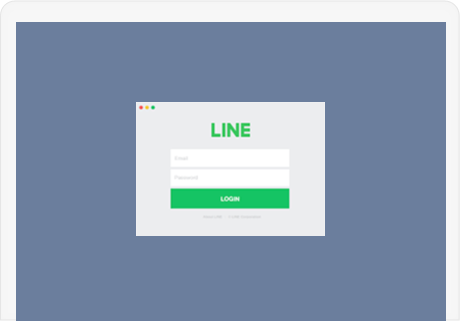
\includegraphics[scale=0.5]{line-login-main-contents.png}  
	\caption[LINE Login]{LINE Login} 
	\label{fig:line-login} 
\end{figure}

LINE Login adalah produk dari LINE yang memungkinkan \textit{developer} membuat aplikasinya menyediakan pilihan \textit{login} melalui akun LINE. Pengguna aplikasi yang dibuat \textit{developer} tidak perlu mendaftar menggunakan \textit{email} dan \textit{password}. \textit{Login} menjadi lebih mudah dan cepat. LINE menyediakan LINE SDK untuk mengintegrasikan LINE Login dengan \textit{native apps}.

\subsection{LINE Bot Designer}

\begin{figure}[H]
	\centering  
	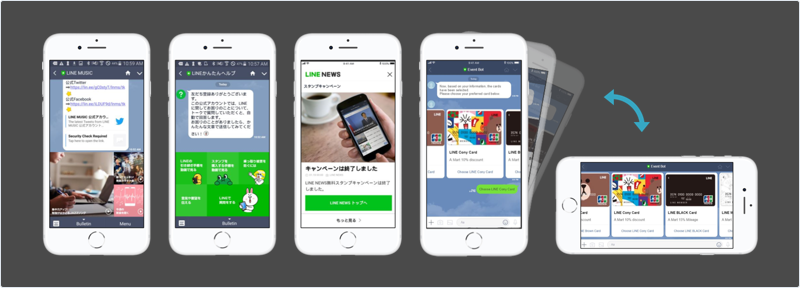
\includegraphics[scale=0.5]{bot-designer.png}  
	\caption[LINE Bot Designer]{LINE Bot Designer} 
	\label{fig:bot-designer} 
\end{figure}

LINE Bot Designer (Gambar~\ref{fig:bot-designer}) adalah produk LINE yang memungkinkan \textit{developer} membuat prototipe LINE bot lebih cepat dan lebih mudah tanpa mengetahui pemrograman. Dengan produk ini, \textit{developer} dapat mendesain \textit{chatbots} sesuai skenario yang diinginkan.

\subsection{Clova}

\begin{figure}[H]
	\centering  
	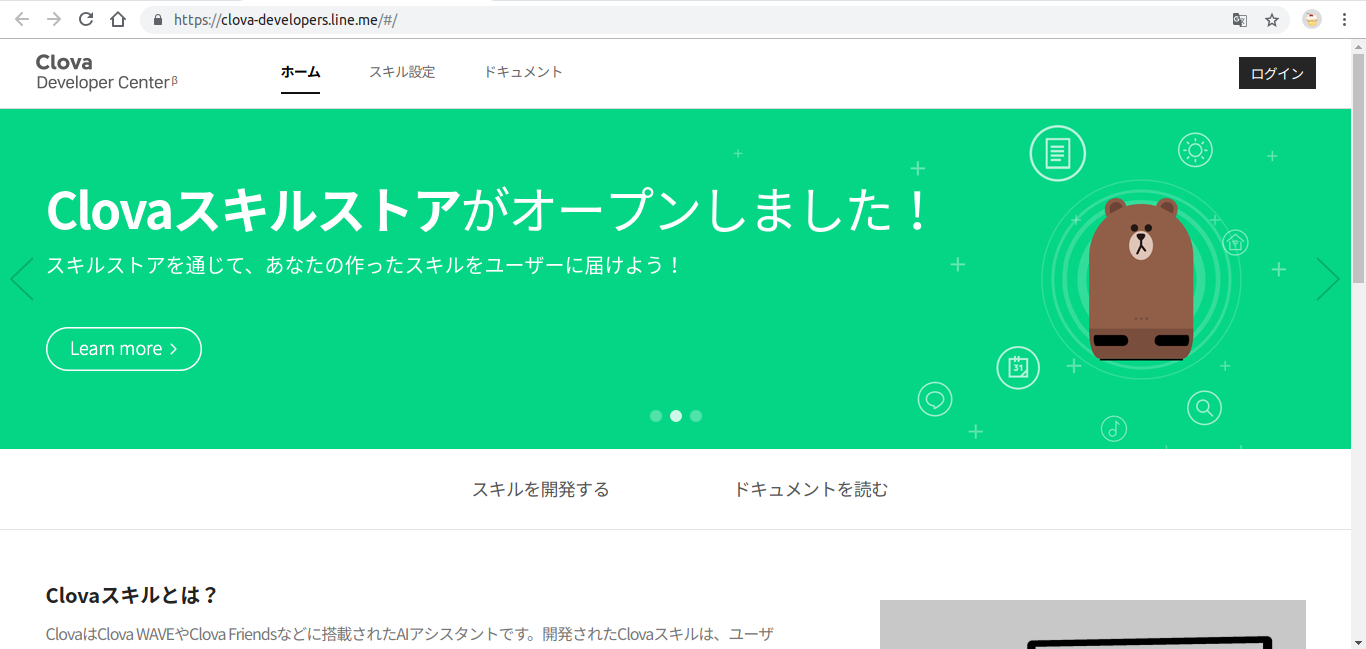
\includegraphics[width=\textwidth]{clova_site.png}  
	\caption[Situs web Clova]{Situs web Clova (https://clova-developers.line.me)} 
	\label{fig:clova_site} 
\end{figure}

Clova adalah sebuah\textit{ AI Assistant} (aplikasi dengan kecerdasan buatan yang berfungsi sebagai asisten) yang dipasang di dalam \textit{Clova Wave} dan \textit{Clova Friends}. Pada saat skripsi ini dibuat, Clova masih dalam tahap pengembangan dan tersedia dalam versi beta. Tidak ada dokumentasi resmi untuk produk ini, tapi ada situs web resminya: \url{https://clova-developers.line.me} (Gambar~\ref{fig:clova_site}). Pada saat skripsi ini ditulis, situs web ini hanya tersedia dalam bahasa Jepang sehingga membutuhkan penerjemah untuk memahami isinya.

\subsection{LINE Pay}
\begin{figure}[H]
	\centering  
	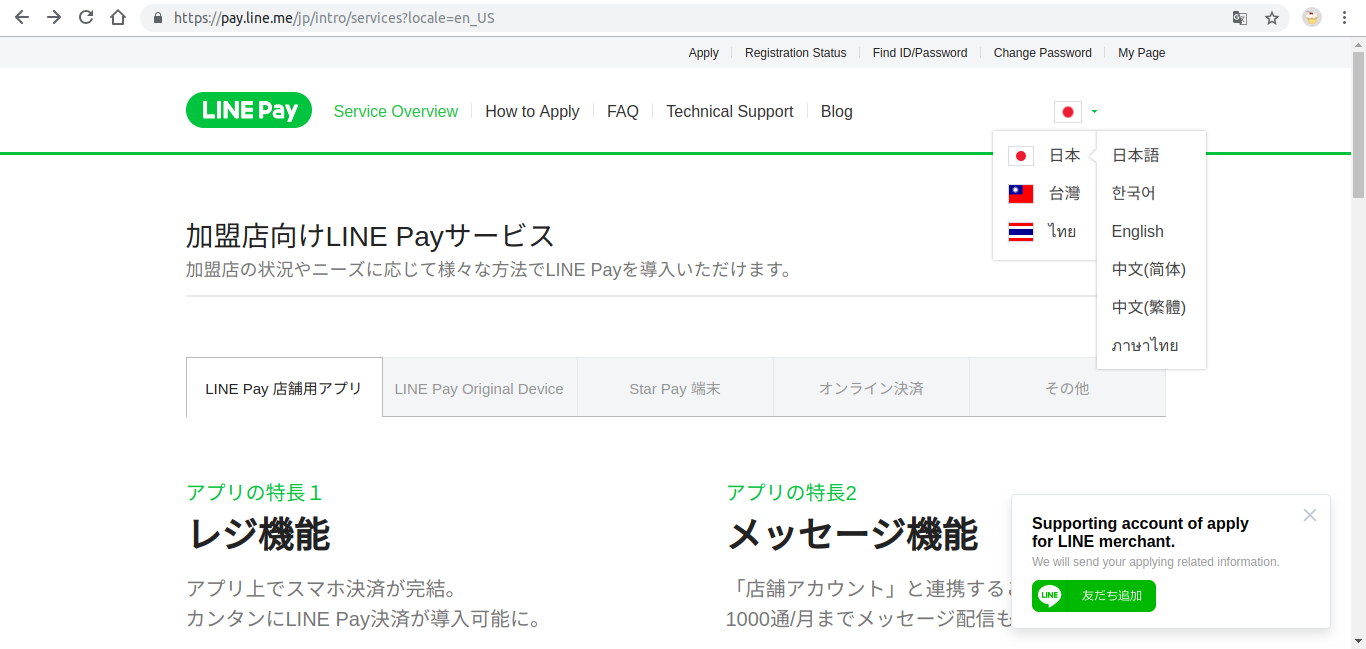
\includegraphics[width=\textwidth]{line_pay_site.png}  
	\caption[Situs web LINE Pay]{Situs web LINE Pay (https://pay.line.me)} 
	\label{fig:line_pay_site} 
\end{figure}

LINE Pay adalah produk LINE yang memungkinkan \textit{developer} mengintegrasikan aplikasi yang dibuat \textit{developer} dengan fitur pembayaran melalui LINE Pay. Tidak ada dokumentasi resmi untuk produk ini, tapi ada situs web resminya: \url{https://pay.line.me} (Gambar~\ref{fig:line_pay_site}). Situs web ini menyediakan informasi LINE Pay di negara Jepang, Republik Tiongkok / Taiwan, dan Thailand. Situs ini tersedia dalam bahasa Jepang, Korea, Inggris, China dengan aksara sederhana, China dengan aksara tradisional, dan Thailand.

\subsection{Messaging API } 
\begin{figure}[H]
	\centering  
	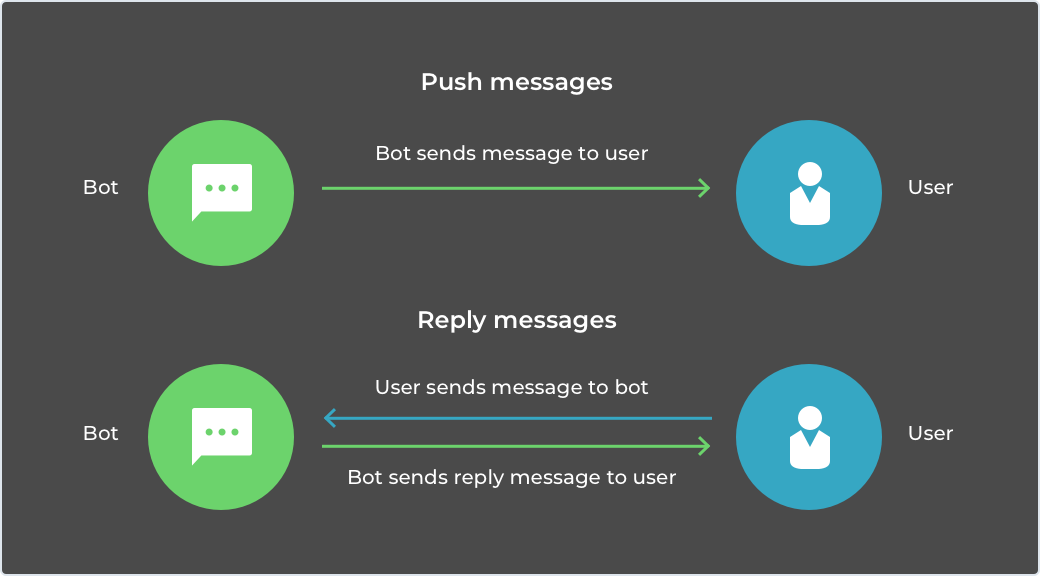
\includegraphics[width=\textwidth]{messaging-api-push-reply-message.png}  
	\caption[Push message dan reply message pada Messaging API]{Messaging API memungkinkan \textit{developer} mengirim push message dan reply message} 
	\label{fig:messaging-api-push-reply-message} 
\end{figure}

Messaging API adalah produk LINE yang memungkinkan \textit{developer} untuk membangun \textit{bot} sebagai sarana komunikasi dua arah antara layanan yang dibangun \textit{developer} dengan pengguna LINE. Dengan Messaging API, \textit{developer} dapat mengirimkan \textit{push message} dan \textit{reply message} (Gambar~\ref{fig:messaging-api-push-reply-message}) ke akun LINE@. \textit{Push message} adalah pesan yang \textit{bot} kirimkan ke pengguna LINE. \textit{Reply message} adalah pesan yang bot kirimkan untuk membalas pesan dari pengguna LINE.

LINE Menyediakan Messaging API untuk membangun messaging bot. Messaging API memungkinkan data dioper antara server dari aplikasi bot dengan LINE Platform. Ketika pengguna LINE mengirimkan pesan ke bot, sebuah \textit{webhook} akan terpicu dan LINE Platform akan mengirimkan permintaan ke URL \textit{webhook bot}. \textit{Server} akan mengirim permintaan ke LINE Platform untuk merespon pengguna. Permintaan akan dikirimkan dalam format JSON. Arsitektur dari Messaging API dapat dilihat pada Gambar~\ref{fig:messaging_api_architecture}.

\begin{figure}[H]
	\centering  
	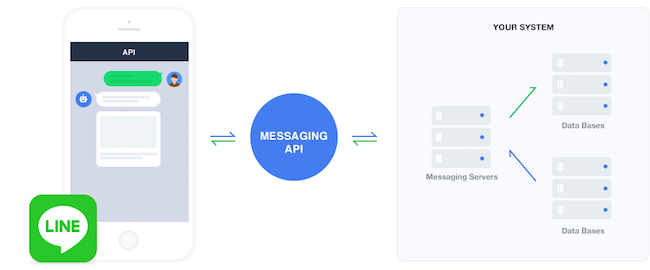
\includegraphics[width=\textwidth]{messaging-api-architecture.png}  
	\caption[Arsitektur Messaging API]{Arsitektur Messaging API} 
	\label{fig:messaging_api_architecture} 
\end{figure}

\textit{Developer} dapat melakukan hal-hal berikut dengan Messaging API :
\begin{itemize}
\item Mengirimkan \textit{reply message}
\item Mengirimkan \textit{push message}
\item Mengirimkan berbagai jenis pesan
\item Mendapatkan profil pengguna yang berinteraksi dengan \textit{bot}
\item Bergabung dengan percakapan grup (\textit{group chats})
\end{itemize}

Untuk menggunakan Messaging API, \textit{developer} memerlukan akun LINE@. Messaging API juga dapat digunakan menggunakan akun resmi/\textit{official accounts}. Akun resmi mendapatkan fitur tambahan untuk pengguna \textit{enterprise}.

\subsubsection{Membuat \textit{Channel}}
Untuk memulai membangun bot dengan Messaging API, \textit{developer} perlu membuat \textit{channel} terlebih dahulu. \textit{Channel} adalah penyambung antara LINE platform dan aplikasi yang dibuat \textit{developer}. Berikut langkah-langkah untuk membuat \textit{channel}:
\begin{enumerate}
\item Langkah ke-1 : Masuk ke LINE Developers \textit{console}

\begin{figure}[H]
	\centering  
	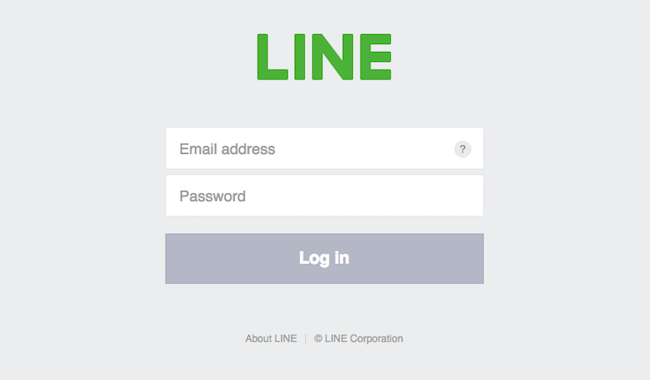
\includegraphics[width=\textwidth]{line-developers-console-login.png}  
	\caption[Tampilan LINE Developers \textit{console} saat login]{Tampilan LINE Developers \textit{console} saat login} 
	\label{fig:line-developers-console-login} 
\end{figure}

\textit{Developer} perlu masuk ke LINE Developers \textit{console} (\url{https://developers.line.me/en/}) dengan alamat \textit{email} dan \textit{password} dari akun LINE \textit{developer} (Gambar~\ref{fig:line-developers-console-login}). Jika \textit{developer} belum memiliki akun LINE, \textit{developer} perlu mengunduh aplikasi LINE untuk mendaftar akun LINE.

\item Langkah ke-2 : Mendaftar sebagai \textit{developer}

\begin{figure}[H]
	\centering  
	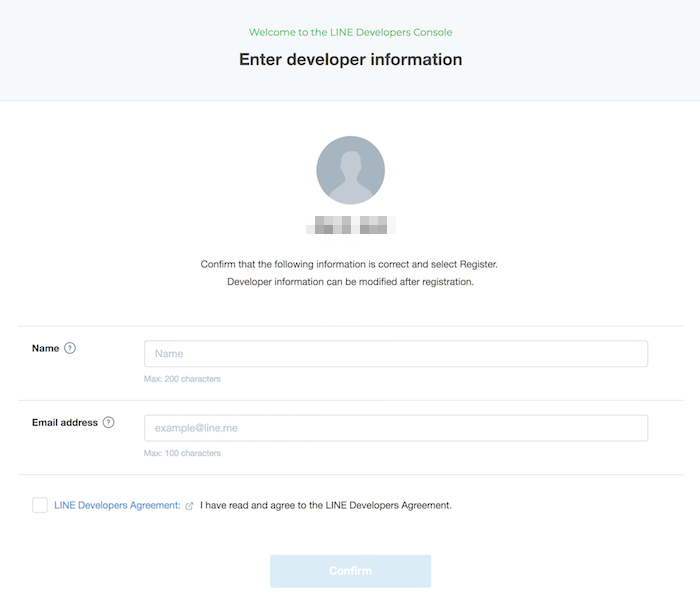
\includegraphics[width=\textwidth]{line-developers-console-register-developer.png}  
	\caption[Tampilan LINE Developers \textit{console} saat \textit{register developer}]{Tampilan LINE Developers \textit{console} saat \textit{register developer}} 
	\label{fig:line-developers-console-register-developer} 
\end{figure}

Apabila \textit{developer} baru pertama kali masuk ke LINE Developers \textit{console}, \textit{developer} perlu membuat akun \textit{developer} (Gambar~\ref{fig:line-developers-console-register-developer}). \textit{Developer} hanya perlu mencantumkan nama dan alamat \textit{email} untuk mendaftar.

\item Langkah ke-3 : Membuat \textit{provider} baru

\textit{Provider} adalah individu atau perusahaan yang menyediakan aplikasi yang akan dibuat. \textit{Developer} perlu mencantumkan nama \textit{provider} untuk membuat \textit{provider} baru. \textit{Developer} dapat menuliskan nama \textit{developer} sendiri atau nama perusahaan \textit{developer}.

\item Langkah ke-4 : Membuat \textit{channel}
\begin{figure}[H]
	\centering  
	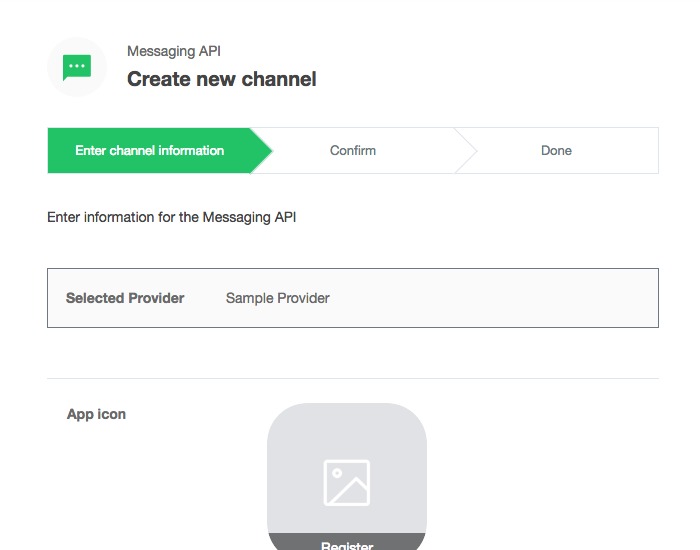
\includegraphics[width=\textwidth]{line-developers-console-create-channel.png}  
	\caption[Tampilan LINE Developers \textit{console} saat membuat \textit{channel}]{Tampilan LINE Developers \textit{console} saat membuat \textit{channel}} 
	\label{fig:line-developers-console-create-channel} 
\end{figure}

\textit{Developer} perlu memasukkan informasi yang dibutuhkan untuk membuat \textit{channel}:
\begin{itemize}
\item Ikon aplikasi

Dokumen gambar untuk ikon aplikasi harus dibawah 3 MB dengan ekstensi JPEG/PNG/GIF/BMP.

\item Nama aplikasi

Nama aplikasi tidak boleh lebih dari 20 karakter. Kata "LINE" tidak dapat digunakan sebagai nama aplikasi, walaupun kapitalisasinya tidak sama. Setelah dikonfirmasi, nama aplikasi tidak dapat diubah untuk tujuh hari ke depan.

\item Deskripsi aplikasi

Deskripsi aplikasi tidak boleh lebih dari 500 karakter.

\item \textit{Plan}

Pada saat mendaftar \textit{channel}, pilihan \textit{plan} yang tersedia hanya dua: \textit{Developer Trial} dan \textit{Free}. \textit{Plan Developer Trial} memungkinkan \textit{developer} untuk membuat bot yang dapat mengirimkan \textit{push message} dan memiliki 50 teman. Apabila \textit{developer} memilih plan ini, maka \textit{developer} tidak dapat melakukan \textit{upgrade} atau membeli ID \textit{premium}. \textit{Plan Free} memungkinkan \textit{developer} untuk membuat bot dengan jumlah teman tak terbatas, tapi \textit{developer} tidak dapat mengirimkan \textit{push message}. \textit{Developer} dapat melakukan \textit{upgrade} kapan saja dengan \textit{plan} ini.

\item Kategori dan Subkategori

\textit{Developer} dapat memilih kategori dan subkategori yang cocok dengan aplikasi yang sedang dikembangkan.

\item Alamat \textit{email}

Alamat \textit{email} yang dicantumkan adalah alamat \textit{email} yang akan menerima notifikasi dan pengumuman penting dari LINE. Maksimal karakter pada alamat \textit{email} adalah 100 karakter.

\end{itemize}

\item Konfirmasi
\begin{figure}[H]
	\centering  
	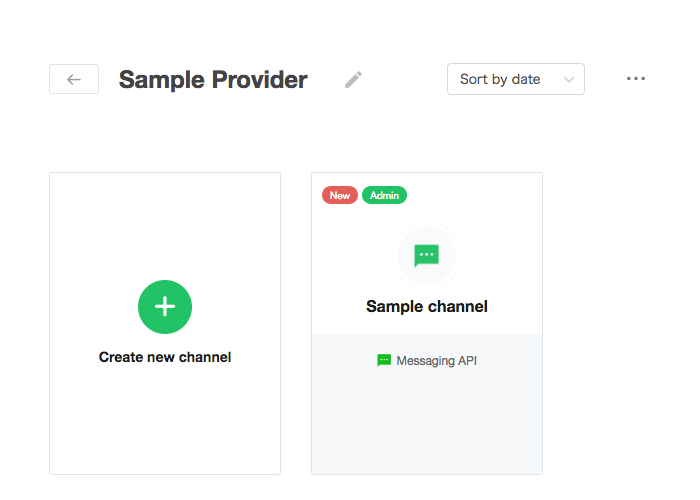
\includegraphics[width=\textwidth]{line-developers-console-confirm-channel.png}  
	\caption[Tampilan LINE Developers \textit{console} saat konfirmasi pembuatan \textit{channel}]{Tampilan LINE Developers \textit{console} saat konfirmasi pembuatan \textit{channel}} 
	\label{fig:line-developers-console-confirm-channel} 
\end{figure}

Konfirmasi \textit{channel} yang baru saja dibuat. Tampilan setelah \textit{channel} dikonfirmasi dapat dilihat di Gambar~\ref{fig:line-developers-console-confirm-channel}.

\end{enumerate}


\subsubsection{Membuat \textit{bot}}
Setelah membangun \textit{channel}, \textit{developer} perlu menyiapkan \textit{server} untuk menjadi \textit{host} dari bot. \textit{Developer} dapat menggunakan layanan \textit{cloud platform}, seperti Heroku. Setelah itu, \textit{developer} dapat mulai mengatur \textit{bot} pada \textit{console}.

Aplikasi \textit{bot} membutuhkan \textit{channel access token} untuk membuat \textit{API call} dan \textit{webhook} URL untuk menerima \textit{webhook payload} dari LINE Platform. \textit{Channel access token} adalah \textit{long-lived token} (token yang tidak memiliki kadaluarsa) yang harus diatur di dalam \textit{authorization header} ketika membuat \textit{API call}. \textit{Developer} dapat menerbitkan lagi \textit{channel access token} kapanpun melalui \textit{console}. Untuk menerbitkan \textit{channel access token}, klik Issue pada "\textit{Channel settings}" di halaman \textit{console}. Sedangkan\textit{ webhook} URL adalah titik akhir dari \textit{server} aplikasi \textit{bot} dimana \textit{webhook payload} dikirimkan.

Untuk mengatur \textit{webhook} URL, \textit{developer} dapat memasukkannya ke halaman \textit{Channel settings} pada \textit{console}. \textit{Webhooks} harus diaktifkan terlebih dahulu dengan menekan tombol \textit{enable webhooks}. Untuk memeriksa apakah \textit{webhook} URL dapat menerima \textit{event webhook}, tekan tombol \textit{Verify} dan pastikan hasilnya \textit{"Success"}. \textit{Webhook} URL harus menggunakan HTTPS dan memiliki sertifikat SSL yang diterbitkan oleh \textit{certificate authority} (CA) yang terotorisasi.

Setelah \textit{token} dan \textit{webhook URL} berhasil diset, tambahkan \textit{bot} sebagai teman melalui akun LINE. \textit{Developer} dapat melakukannya dengan \textit{scan} kode QR pada \textit{Channel Settings}.

\subsubsection{Menkonfigurasi Keamanan}
\textit{Developer} dapat mengkonfigurasi keamanan tapi tidak wajib dilakukan. Untuk meningkatkan keamanan, \textit{developer} dapat mengatur \textit{serve}r yang dapat memanggil API pada LINE Platform pada \textit{Security settings}. \textit{Developer} dapat mendaftarkan alamat IP secara individual atau jika \textit{developer} memiliki \textit{server} yang banyak \textit{developer} dapat menggunakan notasi \textit{Classless Inter-Domain Routing} (CIDR) untuk mendaftarkan alamat jaringan.

\subsubsection{Alur kerja Messaging API}
Ketika \textit{user} berinteraksi dengan \textit{bot} seperti mengirimkan pesan atau menambah \textit{bot} sebagai teman, LINE Platform mengirimkan HTTP POST \textit{request} yang berisi \textit{webhook event object} ke \textit{bot server} yang disebutkan di kolom \textit{"Webhook URL"} pada \textit{console. Request header} berisi \textit{signature.} 

Untuk mengecek apakah \textit{server} dapat menerima \textit{webhook event}, blokir \textit{bot} pada LINE dan cek \textit{server logs} untuk menkorfimasi bahwa \textit{server} dapat menerima \textit{unfollow event} dari LINE Platform.

Untuk memastikan \textit{request} yang dikirim berasal dari LINE Platform, \textit{bot server} harus memvalidasi \textit{X-Line-Signature} pada \textit{request header}. Caranya dengan :
1. Menggunakan \textit{channel secret} sebagai \textit{secret key}, menghasilkan \textit{Base64-encoded digest} dari \textit{request body} menggunakan algoritma HMAC-SHA256
2. Menkonfirmasi \textit{signature X-Line-Signature} dalam \textit{request header} cocok dengan \textit{digest}.
 

\subsubsection{\textit{Webhook Event Object}}
\begin{enumerate}
\item Berikut \textit{webhook event object} khusus untuk \textit{one-on-one chat}:

\begin{itemize}
\item \textit{Message Event}

Menunjukkan bahwa ada \textit{user} yang mengirim pesan. \textit{Event} ini dapat dibalas.

\item \textit{Follow Event}

Menunjukkan bahwa akun \textit{bot} ditambahkan sebagai teman (atau dibuka blokirnya). \textit{Event} ini dapat dibalas.

\item \textit{Unfollow Event}

Menunjukkan bahwa akun bot diblokir

\item \textit{Postback event}

Menunjukkan \textit{user} melakukan aksi \textit{postback}. \textit{Event} ini dapat dibalas.

\item \textit{Beacon event}

Menunjukkan bahwa \textit{user} telah masuk atau keluar dari jangkauan \textit{LINE Beacon}. \textit{Event} ini dapat dibalas.

\item \textit{Account link event }

Menunjukkan bahwa \textit{user} telah menghubungkan akun LINE dengan akun layanan \textit{developer}. 

\end{itemize}

\item Berikut \textit{webhook event object} khusus untuk \textit{group chats}:

\begin{itemize}
\item \textit{Message event}

Menunjukkan bahwa ada \textit{user} yang mengirim pesan. \textit{Event} ini dapat dibalas.

\item \textit{Join event}

Menunjukkan \textit{bot} telah bergabung ke sebuah \textit{group chat}

\item \textit{Leave event}

Menunjukkan \textit{bot} telah keluar dari sebuah \textit{group chat}

\item \textit{Postback event}

Menunjukkan \textit{user} melakukan aksi \textit{postback}. \textit{Event} ini dapat dibalas.

\end{itemize}

\end{enumerate}

\subsubsection{Operasi pada \textit{bot}}
\textit{Developer} dapat melakukan operasi berikut lewat \textit{bot} :
\begin{enumerate}
\item Mengirim \textit{reply message}

\textit{Reply message} adalah pesan yang dikirim sebagai respons dari \textit{user-generated event}. \textit{User-generated event} adalah \textit{event} yang muncul karena user berinteraksi dengan \textit{bot}, misalnya mengirim pesan. \textit{Developer} hanya dapat membalas \textit{webhook events} yang memiliki \textit{reply token}.
Untuk membalas pesan, kirim HTTP POST \textit{request} ke \texttt{/bot/message/reply}. Sertakan \textit{channel access token} di dalam \textit{authorization header} dan \textit{reply token} di \textit{request body}. \textit{Developer} dapat mengirimkan sampai 5 \textit{message object} per \textit{request}.

\item Mengirim \textit{push message}

Untuk mengirim \textit{push message}, \textit{developer} harus memerhatikan \textit{plan} yang dipakai. Apabila \textit{developer} memakai \textit{plan Free} maka \textit{developer} tidak dapat melakukan operasi ini. \textit{Push message} adalah pesan yang dapat \textit{bot} kirimkan ke \textit{user} kapan saja. \textit{Push message} tidak membutuhkan \textit{reply token} seperti saat mengirim \textit{reply message}. Ketika mengirim \textit{push message}, sebutkan \textit{user ID} di dalam \textit{property to}. ID penerima dapat ditemukan dari \textit{webhook event object}. Apabila penerima hanya satu, kirimkan \textit{request} ke \texttt{/bot/message/push}. Sedangkan apabila penerima ada beberapa, kirimkan ke \texttt{/bot/message/multicast}. \textit{Developer} dapat mengirimkan sampai 5 \textit{message object} per \textit{request}.

\item Mendapatkan konten yang dikirim oleh \textit{user}

Untuk mengambil gambar, video, atau audio yang dikirim \textit{user}, kirimkan HTTP GET \textit{request} ke \texttt{/bot/message/{messageId}/content}. Konten yang dikirim oleh \textit{user} otomatis dihapus dalam jangka waktu tertentu.

\item Mendapatkan informasi \textit{user profile}

Untuk mendapatkan informasi \textit{user profile} dari \textit{user} yang menambahkan bot atau mengirim pesan ke bot, kirimkan HTTP GET \textit{request} ke \texttt{/bot/profile/{userId}}. \textit{Request} ini akan mengembalikan \textit{display name, user ID, profile image URL,} dan \textit{status message} (jika tersedia) dari \textit{user}.
\end{enumerate}

\subsection{LINE@ Manager}
LINE@ Manager adalah alat untuk mengatur akun LINE@ (LINE bot). \textit{Developer} dapat meningkatkan \textit{user experience} dengan mengatur halaman akun, membuat \textit{Timeline post}, dan menggunakan fitur lain yang disediakan LINE@ Manager. Berikut adalah hal-hal yang bisa dilakukan:
\begin{enumerate}
\item Mengubah tampilan halaman akun

\textit{Developer} dapat mengubah gambar cover, logo, tombol, dan informasi yang disediakan

\item Mengatur \textit{greeting message}

Jika \textit{developer} mengaktifkan \textit{greeting message} pada \textit{Channel settings}, maka \textit{developer} dapat mengatur \textit{greeting message} yang akan dikirim ke \textit{user} saat pertama kali menambahkan bot sebagai teman. \textit{Developer} dapat melakukannya juga dengan program melalui \textit{follow webhook event}.

\item Mengatur \textit{auto reply message}

Jika \textit{developer} mengaktifkan "\textit{Auto reply message}" pada \textit{Channel settings}, maka \textit{developer} dapat mengatur pesan balasan otomatis setiap \textit{user} mengirimkan pesan ke bot.
\end{enumerate}